\chapter{ALGORITHM SELECTION AND HYPERPARAMETER OPTIMIZATION BASED QUANTIFICATION OF ERROR CONTRIBUTION IN IMAGE CLASSIFICATION PIPELINES}
\label{chap:EP}

\let\thefootnote\relax\footnotetext{}

%%%%%%%%%%%%%%%%%%%%%%%%%%%%%%%%%%%%%%%%%%%%%%%%%%%%%%%%%%%%%%%%%%%%%%%%%%%%%%
%\section{Introduction and Motivation}
%%%%%%%%%%%%%%%%%%%%%%%%%%%%%%%%%%%%%%%%%%%%%%%%%%%%%%%%%%%%%%%%%%%%%%%%%%%%%%

\section{Introduction} 
\label{sec1}
Machine learning and data science has entered many domains of human effort in modern times. The number of self-reported data scientists has doubled in recent years \cite{harrison1995validity}. They have entered various domains including academia, industry and business among others. There has therefore been a demand for machine learning tools that are flexible, powerful and most importantly interpretable. The effective application of machine learning tools unfortunately requires an expert understanding of the frameworks and algorithms that are present in a machine learning pipeline. It also requires knowledge of the problem domain and understanding of the assumptions used in the analysis. In order for these tools to be used adequately by non-experts; additional tools must be developed for understanding and interpreting the results of the application of a data analytic pipeline on a domain specific problem.  

\begin{figure}[ht!]
    \centering
    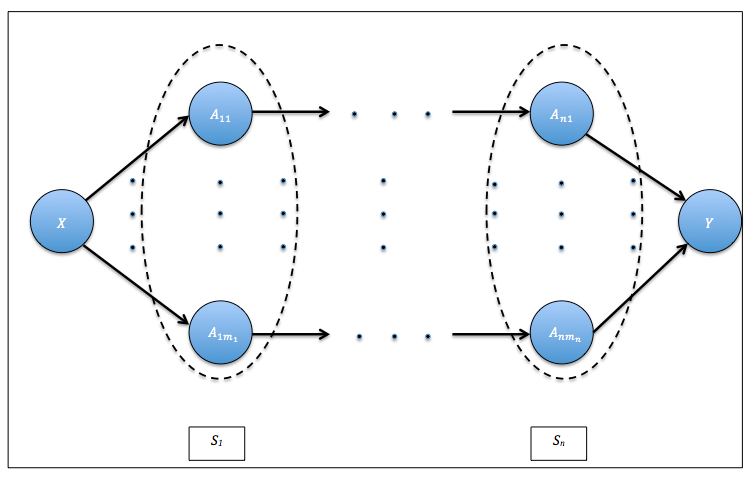
\includegraphics[scale=0.5]{img/EP/generalized_pipeline}
    \caption{Representation of a machine learning pipeline}
    \label{fig:pipeline}
\end{figure}

Pipelines in machine learning and data science are commonly organized in the form of interdependent components. Such components that make up a data analytic pipeline include data preprocessing, feature extraction, feature transformation like dimensionality reduction, model building and model evaluation among others. Such pipelines provide a natural way to organize such tasks, and they play a key part in the design and implementation of large scale data science projects. Machine learning toolboxes like scikit-learn \cite{pedregosa2011scikit}, RapidMiner \cite{mierswa2006yale} and Apache Spark \cite{spark2016apache} independently provide frameworks for implementing pipelines. Fig. \ref{fig:pipeline} shows a generic representation of data analytic pipelines. Each computational step of the pipeline $S_{i}$ consists of several algorithms ($A_{ij}$) to choose from. Each algorithm in the pipeline consists of its own hyperparameters $\theta_{ijk}$ that must be optimized for using the algorithm. Therefore, there are an exponential number of combinations of algorithms and hyperparameters in a given analytic pipeline skeleton. This then is an extremely computationally intensive task of optimizing the pipeline. Tuning this pipeline can be viewed as the optimization of a blackbox objective function that is noisy and expensive to evaluate. The input to the blackbox are the input dataset $X$, the pipeline $P$(consisting of the steps $S_{i}$, the algorithms $A_{ij}$ and corresponding hyper-parameters $\theta_{ijk}$) and the output performance $Y$ such as validation error, accuracy, F1-score and cross-entropy loss among others, which are examples of the objective function.The goal of a data scientist is to find the best set of algorithms and hyper-parameters in this pipeline that optimizes the objective function. This corresponds to finding an optimal path through the pipeline in \ref{fig:pipeline}.  Simple methods such as grid and random search \cite{bergstra2012random} have been used to tackle this problem. More complicated approaches such as Bayesian optimization \cite{snoek2012practical, zhang2016flash} have been used successfully for approaching more difficult problems. Pipeline optimization as a whole has also been approached using genetic algorithms \cite{olson2016evaluation, olson2016tpot, olson2016automating}.
We use grid search, random search and bayesian optimization methods for optimization of the pipeline and each individual path in it.  

Interpretation of machine learning pipelines is extremely important for their adoption in various domains. Domain experts do not prefer the use of black-box pipelines. They would prefer to understand how predictive decisions are made by the pipeline. Recently there has been an advent of models and techniques for improving the interpretability of machine learning. \cite{ribeiro2016model} introduces a model-agnostic method for interpreting machine learning blackboxes. \cite{doshi2017towards} attempts at a definition of interpretability in this context and how it should be measured. \cite{koh2017understanding} uses influence functions to understand blackbox predictions. In this work, we attempt to provide an interpretation of machine learning pipelines as a whole as opposed to the approaches which are geared toward interpretation of individual machine learning algorithms in general. This includes understanding the predictions with respect t other components like feature extraction and feature transformation and also to smaller components like individual hyper-parameters. To our knowledge, this type of approach to interpretation has not been done before.
To this end, we propose the understanding of the contribution of error in data analytic pipelines. We use the cross-entropy loss as the performance metric of the optimization algorithms and basis of error quantification in the image classification pipelines. Understanding the source of the error in the predictive model is important for experts to design the data analytic pipelines. Experts can use the information from error contributions to focus attention on certain parts of the pipeline depending on the source of error. In addition, it also provides non-experts in machine learning insight into the predictions of the model. They can understand whether the error they are seeing are due to which component of the process. We introduce a methodology to quantify the contribution of error from different components of the data analytic pipeline, namely the computational steps and algorithms in the pipeline. 
% In addition, a model of error propagation is proposed in this work. This model represents the propagation of error from the computational steps in the pipeline starting from the first step that could be data preprocessing in Fig. 1 to the last step that is usually learning algorithms in a machine learning problem.  

Pipeline optimization algorithms like grid search, random search \cite{bergstra2012random} and Bayesian optimization \cite{snoek2012practical} are used to optimize the pipeline for performing experiments with the error quantification and propagation methodology. We take two different approaches to optimization. The first is hyper-parameter optimization (HPO) where a computational path in Fig. \ref{fig:pipeline} is optimized. This is equivalent to a combined optimization of the hyperparameters of the algorithms on that path. The second type of optimization is denoted as combined algorithm selection and hyperparameter optimization (CASH). This is a more difficult problem, because the pipeline is optimized globally, in that the result of the optimization is a single optimized path that produces the best performance over all the paths in the machine learning workflow.  

We use four datasets to demonstrate the error quantification and propagation methodology. The machine learning problem is that of image classification. We show the performance of both the optimization frameworks (HPO and CASH) for the experiments. We show experimentally that CASH using random search can be efficiently used for quantification of errors from the different computational steps of the pipeline. In addition, HPO frameworks of both Bayesian optimization and random search provides  estimates of error contributions from the algorithms and hyperparameters in a particular path of the pipeline.
% We use the computationally efficient CASH framework of random search to perform experiments on the error propagation model. 
We demonstrate from the results that the error quantification methodology maybe used by both data science and domain experts to improve and interpret the results of image classification pipelines.  

The paper is organized as follows. Section \ref{sec2} describes the methods that are used in this work and the proposed methodology of error contribution. The experimental frameworks, datasets, results and discussion makes up section \ref{sec3}. This is followed by the conclusion in section \ref{sec4}.

\section{Foundations}
\label{sec2}
In this section we describe the optimization problem and the black-box optimization methods that are used in this work. 
\subsection{Algorithm selection and hyper-parameter optimization}
\label{subsec_AS_HPO}
We approach the problem of optimization of the pipeline from two frameworks. In one framework, each path in the pipeline in \ref{fig:pipeline} is individually optimized. This essentially boils down to problem of hyper-parameter optimization (HPO)  because the hyperparameters of each algorithm are optimized for each individual path. In the second framework, the entire pipeline is optimized. This means that the algorithms and hyperparameters are optimized together. This is denoted as combined algorithm selection and hyper-parameter optimization (CASH).

\subsubsection{Hyper-parameter optimization (HPO)}
\label{subsubsec_HPO}
Let the \textit{n} hyperparameters in a path be denoted as $\theta_1, \theta_2, ..., \theta_n$, and let $\Theta_1, \Theta_2, ..., \Theta_n$ be their respective domains. The hyperparameter space of the path is  \textbf{$\Theta$} = $\Theta_1 \times \Theta_2 \times ... \times \Theta_n$.


When trained with $\emph{$\theta$} \in \textbf{$\Theta$}$ on data $D_{train}$, the validation error is denoted as \par
\noindent $\mathcal{L}(\theta, D_{train}, D_{valid})$. Using $k$-fold cross-validation, the hyperparameter optimization problem for a dataset $D$ is to minimize:
\begin{equation}
\label{hpo}
f^D(\theta) = \frac{1}{k}\sum_{i=1}^{k} \mathcal{L}(\emph{$\theta$}, D_{train}^{(i)}, D_{valid}^{(i)}) 
\end{equation}
Hyperparameters $\theta_i$ may be numerical, categorical or conditional with a finite domain. The minimization of this objective function provides the optimal configuration of hyperparameters on a particular path in the pipeline in Fig. \ref{fig:pipeline}.

\subsubsection{Combined algorithm selection and hyper-parameter optimization (CASH)}
\label{subsubsec_CASH}
We can define the CASH formulation using Fig. 1. Let there be $n$ computational steps in the pipeline. Each step $i$ in the pipeline consists of algorithms $A_i(\Theta_i)$, where $A_i(\Theta_i) = \{A_{i1}(\theta_{i1}), ..., A_{im_{i}}(\theta_{im_{i}})\}$, $m_{i}$ is the number of algorithms in step $i$, $A_{ij}$ represents the $j$-th algorithm in step $i$, and \textbf{$\theta_{ij}$} represents the set of hyperparameters corresponding to  $A_{ij}$. The entire space of algorithms and hyperparameters is therefore given by \par
\noindent $\mathcal{A} = A_1(\Theta_1) \times A_2(\Theta_2) \times ... \times A_n(\Theta_n)$. The objective function to be minimized for CASH is given by
\begin{equation}
\label{cash}
f^D(A) = \frac{1}{k}\sum_{i=1}^{k} \mathcal{L}(\emph{A}, D_{train}^{(i)}, D_{valid}^{(i)}) 
\end{equation}
where, $A \in \mathcal{A}$ and other notations are the same as those introduced in the previous section.

\subsection{Optimization methods}
The critical step in HPO or CASH is to choose the set of trials in the search space, which is $\Theta$ for HPO and $\mathcal{A}$ for CASH. In this section, methods that are used in this paper for optimization of Eq. \ref{hpo} and Eq. \ref{cash} are described. Grid search, random search and Bayesian optimization are used in this work.
\subsubsection{Grid search}
\label{subsubsec1}
Grid search is the simplest of all methods for coming up with trials in the search space. The set of trials in grid search is formed by assembling every possible set of values in $\Theta$ and $\mathcal{A}$ and computing the validation loss for each. The configuration $\theta \in \Theta$ or $A \in \mathcal{A}$ that minimizes the validation loss $\mathcal{L}$ is chosen as the optimum configuration. Unfortunately grid search is computationally very expensive. For HPO, the number of trials corresponds to $\prod_{i=1}^n |\Theta_i|$, and for CASH this is $\prod_{i=1}^n |A_i(\Theta_i)|$. This product makes grid search suffer from the \textit{curse of dimensionality}. This is because the number of trials grows exponentially with the number of hyperparameters. However, grid search has certain advantages. Firstly, parallelization and implementation is trivial. In addition, grid search is robust in the sense that results maybe replicated easily. 

\subsubsection{Random search}
\label{subsubsec2}
Random search is the optimization method where trial configurations are randomly sampled from the search space of HPO ($\Theta$) or CASH ($\mathcal{A}$). \cite{bergstra2012random} shows empirically and theoretically that randomly selecting trials is sufficiently accurate and more efficient than performing optimization using grid search. We also show similar results in this work.

\subsubsection{Bayesian optimization}
\label{subsubsec1}
Sequential model based Bayesian optimization (SMBO) \cite{hutter2011sequential} is the method of choice when it comes to optimization of complicated black-box functions. In a nutshell, it consists of two components. The first is a probabilistic model and the second is an acquisition function. The probabilistic model can be modelled using Gaussian processes (Spearmint) \cite{snoek2012practical}, random forests (SMAC) \cite{hutter2011sequential} and using density estimation with Tree-structured Parzen estimators (TPE) \cite{bergstra2011algorithms}. The acquisition function determines the future candidates or trials for evaluation. The acquisiton function is relatively cheap to evaluate compared to the actual objective function $f^D$. One of the most prominent acquisition functions is \textit{expected improvement} (EI) \cite{expected_improvement}. We use the sequential model-based algorithm configuration (SMAC) that uses random forests as the Bayesian optimization framework. This is because it can be used for optimizing conditional hyperparameter configurations, and based on empirical results in \cite{eggensperger2013towards}.

\section{Proposed methods}
\label{sec3}
In this section the proposed methodology for quantification of error contribution is presented. The method is independent of the black-box optimization methods that maybe used for both the HPO and CASH formulations.

\subsection{Error contribution with the agnostic methodology}
\label{EQ}
Machine learning pipelines maybe understood and interpreted by quantifying the contribution of error from different parts of the pipeline. For example, it is useful for machine learning experts and domain experts to understand and identify where the source of the error is in a pipeline. Referring back to Fig. \ref{fig:pipeline}, if it was known that most of the error in the final result originated from feature extraction, then machine learning practitioners would devote more time and energy to coming up with better algorithms for feature extraction or fine-tuning the algorithms in that step to reduce the error. In addition, if it were possible to quantify the contribution of errors from certain algorithms or hyper-parameters in the pipeline, then the data scientists would try to fine tune the algorithms in the pipeline or even try to replace the algorithms with better alternatives. 

We propose an \textit{agnostic} methodology for quantifying error contributions from different parts of the pipeline. It is quantified as the minimum error obtained by being agnostic to a particular component of the pipeline (computational step or algorithms). We shall define what \textit{agnostic} refers to for both computational steps and algorithms individually.

\subsubsection{Quantification of error from computational steps}
\label{subsubsec_eq_steps}
The \textit{agnostic} methodology maybe used for quantification of error contributions from computational steps like feature extraction, data pre-processing and and learning algorithms. Being \textit{agnostic} to a computational step means that the algorithms in that step are selected randomly for that step while the remaining pipeline is optimized. The average of the minimum errors obtained with each algorithm in the step used as the only algorithm in that particular step, provides an estimate of the agnostic error from a particular pipeline.  
More formally, the agnostic methodology is implemented for computational steps in the following manner. Using \ref{fig:pipeline} as a reference, let $n$ be the number of steps in the pipeline. Each step in the pipeline is denoted as $S_i$. $|S_i|$ is the number of algorithms in step $i$. $A_{ij}$ denotes the $j$-th algorithm in the $i$-th step. $E^*$ represents the minimum validation error found after optimization of the entire pipeline (using the CASH framework). $E_{A_{ij}}^*$ is the minimum  validation error found with $A_{ij}$ as the only algorithm in step $i$. The error contribution from step $i$, $EC_{S_i}^*$ is given by Eq. \ref{eq_step}.
\begin{equation}
\label{eq_step}
EC_{S_i}^* = \frac{1}{|S_i|}\sum_{z=1}^{|S_i|} E_{A_{ij}}^* - E^*,
\end{equation}
where, $i = {1, ..., n}, j = {1, ..., |S_i|}$
Taking the difference with respect to the global minimum in Eq. \ref{eq_step} provides an estimate of the error contribution from step $i$ of the pipeline. A large value of $EC_{S_i}^*$ would mean that step $S_i$ is important for the pipeline.

\subsubsection{Quantification of error from algorithms}
\label{subsubsec_eq_alg}
The \textit{agnostic} methodology for algorithms is implemented as follows. Similar to the \textit{agnostic} methodology for steps defined above, we define the \textit{agnostic} methodology for algorithms. In this case, we focus on a single path in the pipeline in Fig. 1. Let's assume we are trying to quantify the error contribution of a particular algorithm $A_{ij}$ that lies on path $p$. Being $agnostic$ to $A_{ij}$ means we optimize everything else on the path except the algorithm. This means that we pick the hyperparameters $\theta_{ij}$ of algorithm $A_{ij}$ randomly while optimizing the rest of the algorithms on the path. This is formally calculated by taking the average of the optimum errors on the path for each configuration of $\theta_{ij}$. The minimum validation error on the path is then subtracted from this error to give us the error contribution from algorithm $A_{ij}$ on path $p$. These errors are computed using the results and the search trials on the CASH framework in section \ref{subsubsec_CASH}.

\begin{equation}
\label{eq_alg}
EC_{A_{ij}}^* = \frac{1}{|\theta_{ij}|}\sum_{z=1}^{|\theta_{ij}|} {E_{A_{ij}}^z}^* - {E_{A_{ij}^p}^*},
\end{equation}

where, $i = {1, ..., n}, j = {1, ..., |\theta_{ij}|}$, $|\theta_{ij}|$ represents the number of hyperparametric configurations of $A_{ij}$,  ${E_{A_{ij}}^z}^*$ is the minimum error obtained with the $z$-th configuration of $\theta_{ij}$ and $E_{A_{ij}^p}^*$ is the minimum error found over the path $p$ that consists of algorithm $A_{ij}$.


\subsubsection{Quantification of error from hyper-parameters}
\label{subsubsec_eq_hyper}
The \textit{agnostic} methodology for hyper-parameters is implemented as follows. In the case of hyper-parameters, we focus on a single path similar to what we did for algorithms. Let's assume we are trying to quantify the error contribution of a particular hyper-parameter $\theta_{ijk}$ that lies on path $p$, i.e. the $k$-th hyper-parameter of the $j$-th algorithm in the $i$-th step of the pipeline. Being $agnostic$ to $\theta_{ijk}$ means we optimize everything else on the path except the hyper-parameter. This means that we pick the hyperparameter $\theta_{ijk}$ of algorithm $A_{ij}$ randomly while optimizing the rest of the hyper-parameters on the path. This is formally calculated by taking the average of the optimum errors on the path for each configuration of $\theta_{ijk}$. The minimum validation error on the path is then subtracted from this error to give us the error contribution from hyper-parameter $\theta_{ijk}$ on path $p$. This is again computed using the HPO framework described in section \ref{subsubsec_HPO}.

\begin{equation}
\label{eq_hyper}
EC_{\theta_{ijk}}^* = \frac{1}{|\theta_{ijk}|}\sum_{z=1}^{|\theta_{ijk}|} {E_{\theta_{ijk}}^z}^* - {E_{A_{ij}^p}^*},
\end{equation}

where, $i = {1, ..., n}, j = {1, ..., |\theta_{ij}|}$, k = number of hyper-parameters of algorithm $A_{ij}$. $|\theta_{ijk}|$ represents the number of configurations of $\theta_{ijk}$,  ${E_{\theta_{ijk}}^z}^*$ is the minimum error obtained with the $z$-th configuration of $\theta_{ijk}$ and $E_{A_{ij}^p}^*$ is the minimum error found over the path $p$ that consists of algorithm $A_{ij}$.

% The above method for quantification of error is slightly limited in the sense that it only returns non-zero values for algorithms that are in the optimum path (with respect to paths in \ref{fig:pipeline}) that corresponds to the minimum error found. The following method redresses this problem. Similar to the \textit{agnostic} method used for steps, the corresponding method is when the algorithm itself is taken to be \textit{agnostic}. This means that everything except the algorithm is optimized, and the hyper-parameters of the algorithm is randomly sampled. This error may be estimated by taking the average of minimum errors in the paths that the algorithm is involved in. This is because, if we are agnostic to a particular algorithm, the path through the algorithm is not optimized and we are randomly select any path that the algorithm is involved in with respect to \ref{fig:pipeline}. The error contribution of the algorithm is therefore given by the difference between this error and the minimum error found over all the paths that the algorithm is involved in. This notion is formalized as $EC_{A_{ij}}^*$ in Eq. \ref{eq_alg2}.
% \begin{equation}
% \label{eq_alg2}
% EC_{A_{ij}}^* = \frac{1}{|A_{ij}^p|}\sum_{j=1}^{|A_{ij}^p|} {E_{A_{ij}}^k}^* - E_{A_{ij}}^*,
% \end{equation}
% where, $|A_{ij}^p|$ is the number of paths in the pipeline that algorithm $A_{ij}$ is involved in. ${E_{A_{ij}}^k}^*$ is the minimum error found over the $k$-th path that the $A_{ij}$ is involved in. $E_{A_{ij}}^*$ is the minimum error over all the paths that go through $A_{ij}$.
% \subsection{Error propagation}
% \label{subsec2}
% Understanding how error propagates along a machine learning pipeline is important for it's analysis. The final error that is obtained in a pipeline consists of two sources. The first is the actual error that originates from the various components of the pipeline. The second is the error that is accumulated along the pipeline because of the propagation or the propagated error. For example an algorithm like principal components analysis that is used for transforming the features may provide a better performance with one feature extraction algorithm over another. Data scientists and domain experts alike may use this tool to understand and analyze a pipeline in detail to make sense of how the error propagates. This difference in performance maybe attributed to propagation. We propose a method to model the error propagation for both algorithms and steps using the error contributions computed using the formulation in the previous section. This is done by introducing \textit{naive} algorithms at each step of the pipeline. This model is represented in Fig. \ref{fig:naive}. 
% \begin{figure}[H]
% \label{naive_pipeline}
%     \centering
%     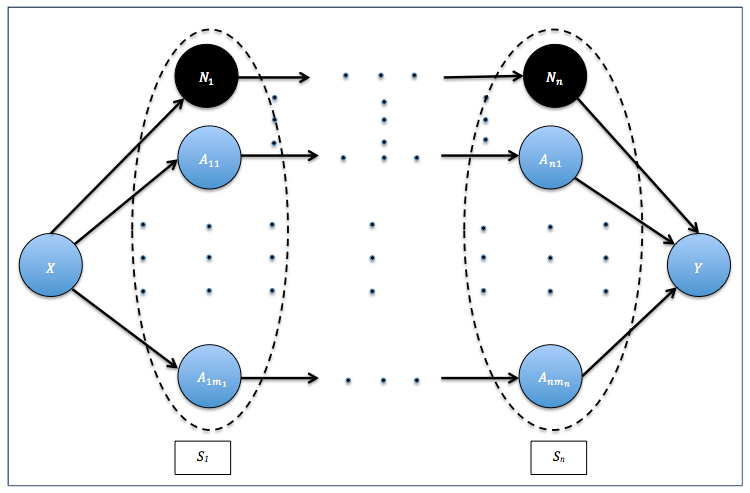
\includegraphics[scale=0.5]{generalized_naive}
%     \caption{Naive methodology used in the error propagation model}
%     \label{fig:naive}
% \end{figure}
% As shown in the figure above, \textit{naive} algorithms are introduced at each step. The are denoted as $N_i$.This naive formulation is an integral component for the error propagation model. The assumption we make is that all of the error that is made by the naive algorithms is because of the algorithm itself and no error is propagated because of it. We can therefore define 6 different types of errors using this approach. These errors are represented in Table 1.


% \begin{table}[h!]
% \centering
% \caption{Notations for error definitions used in the error propagation model}
% \begin{tabular}{ |m{6em}|m{10cm}| } 
%  \hline
%  Notation & Definition \\ 
%  \hline
%  $E_{opt->opt}$ & Minimum error found by using the optimum algorithm or hyperparameter the current step or algorithm respectively and all the steps or algorithms that proceed it. \\ 
%  \hline
%  $E_{agnostic->opt}$ & Minimum error found by using the $agnostic$ methodology for the current step or algorithm and optimizing all the steps or algorithms that proceed it. \\ 
%  \hline
%   $E_{naive->opt}$ & Minimum error found by using the naive algorithm for the current step or algorithm and optimizing all the steps or algorithms that proceed it. \\ 
%  \hline
%  $E_{opt->naive}$ & Minimum error found by using the optimum algorithm or hyperparameters for the current step or algorithms respectively and naive algorithms for all the steps or algorithms that proceed it. \\ 
%  \hline
%  $E_{naive->naive}$ & Minimum error found by using the naive algorithm for the current step or algorithm and naive algorithms all the steps that proceed it. \\ 
%  \hline
%  $E_{agnostic->naive}$ & Minimum error found by using the $agnostic$ methodology for the current step or algorithm and naive algorithms all the steps that proceed it.\\ 
%  \hline
%  \end{tabular}
% \label{table:1}
% \end{table}

% Let us now define 3 types of error contributions using the notations in Table 1.
% \begin{equation}
% \label{ep_errors}
% \begin{aligned}
% \Delta E_1 =& E_{agnostic->opt} - E_{opt->opt} \\
% \Delta E_2 =& E_{agnostic->naive} - E_{opt->naive} \\ 
% \Delta E_3 =& E_{naive->naive} - E_{naive->opt}
% \end{aligned}
% \end{equation}
% Eq. \ref{ep_errors} represents the error contributions from each step of the pipeline using the naive and agnostic methodology. $\Delta E_1$ is the same as the error contribution $EC_{S_i}$ for steps or $EC_{A_{ij}}$ for algorithms. described in Section 3.1. It is the error contribution from a particular step or algorithm with respect to the pipeline or path respectively. $\Delta E_2$ is the error contribution from a step or algorithm with naive algorithms in the steps proceeding it. This value represents the error contribution without error propagation. $\Delta E_3$ is the quantification of the actual error that is added by the naive algorithms.  Let us define the actual error contributed by a step or algorithm as $\alpha$ and the propagated error as a multiple of the actual error. Let this be denoted as $\gamma\alpha$. We denote $\gamma$ as the \textit{propagation factor}.  Then we can write $\Delta E_1$ as,
% \begin{equation}
% \Delta E_1 = \alpha + \gamma\alpha
% \end{equation}
% Similarly, $\Delta E_2$ consists of the actual error from the step or algorithm and the propagated error. The propagated error is a multiple of the actual error and the error added by the naive algorithms. Therefore, we can formalize this as:
% \begin{equation}
% \Delta E_2 = \alpha + \gamma(\alpha + \Delta E_3)
% \end{equation}
% Let as denote the actual error as $E_{direct}$ which is the same as $\alpha$, and the propagated error as $E_{propagation}$ which is $\gamma\alpha$. Solving Eq. 7 and Eq. 8 simultaneously, we get the values for $E_{direct}$, $E_{propagation}$ and the \textit{propagation factor} $\gamma$
% \begin{equation}
% \begin{aligned}
% E_{direct} =& \frac{\Delta E_1 \Delta E_3}{\Delta E_2 + \Delta E_3 - \Delta E_1} \\
% E_{propagation} =& \frac{\Delta E_1 (\Delta E2 - \Delta E_1)}{\Delta E_2 + \Delta E_3 - \Delta E_1}\\
% \gamma =& \frac{\Delta E_2 - \Delta E_1}{\Delta E_3}
% \end{aligned}
% \end{equation}

 

\section{Experiments and results}
\label{sec4}
In this section, we describe the experiments performed on the data analytic pipeline to quantify the error contributions and propagation from different components of the pipeline. Image classification is the data analytic problem chosen for demonstrating the error quantification experiments. A representation of an image classification pipeline is shown in Fig. \ref{fig:flowchart} in the form of a flowchart.  
\begin{figure}[ht!]
    \centering
    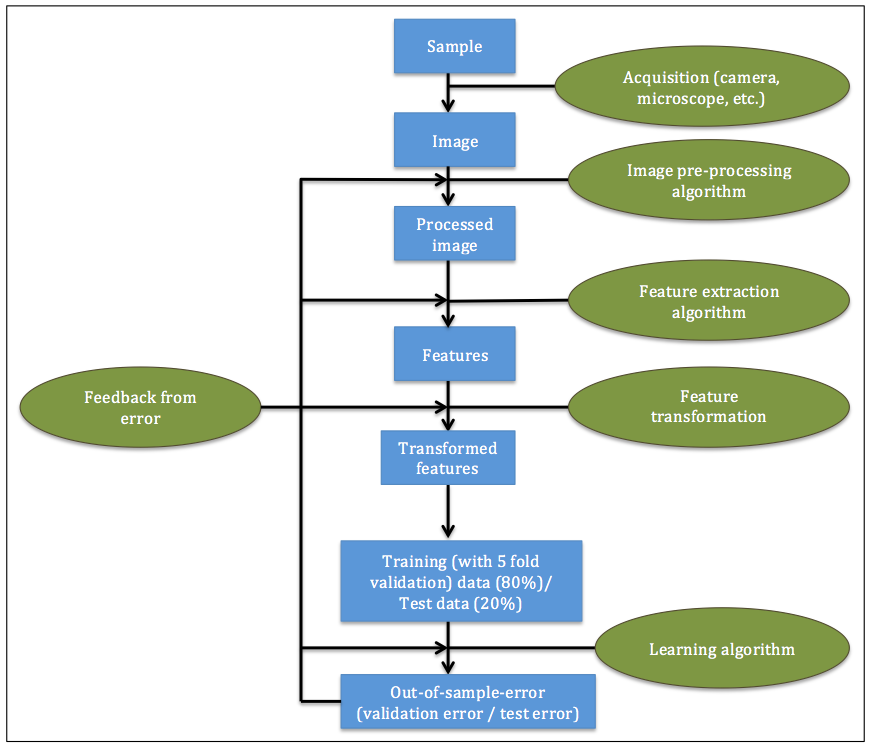
\includegraphics[scale=0.4]{img/EP/flowchart}
    \caption{Representation of an image classification pipeline. The pipeline consists of the steps represented by green ellipses and the outputs of each step represented by blue rectangles. In this work, we focus on the steps and outputs after pre-processing.}
    \label{fig:flowchart}
\end{figure}
In this work, we focus on real world scientific datasets from the domains of medical pathology and material science.  Therefore, the flowchart starts with a sample that is imaged with acquisition technology like a camera or a microscope. The image is then processed using image pre-processing algorithms like normalization and standardization. This may also include image segmentation algorithms. This is followed by feature extraction algorithms that extract useful information from the images. Sometimes, the features extracted are transformed to a different vector space using feature transformation (feature selection or dimensionality reduction) algorithms. The dataset is then divided into training and test datasets in a 80-20 split. Finally, classification algorithms like random forests \cite{breiman2001random} and support vector machines (SVM) \cite{cortes1995support} are used for learning in order to build a predictive model for the image classification problem. The performance of the pipeline is evaluated using classification metrics like F1-score, accuracy, precision and recall. We use the cross entropy loss on the validation data as the estimate of the out-of-sample error. This error is then used as a feedback to quantify the contribution of the errors from different components of the pipeline. The specific pipeline used in this work is shown in the following figure.

\begin{figure}[ht!]
    \centering
    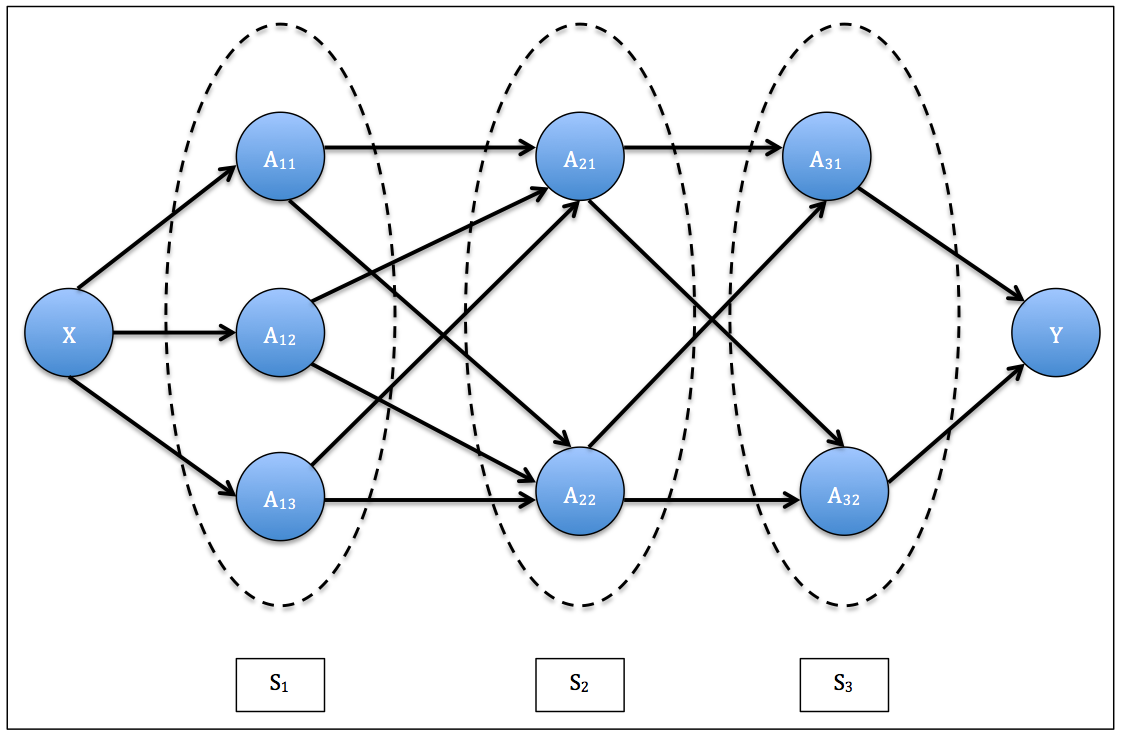
\includegraphics[scale=0.3]{img/EP/pipeline}
    \caption{Representation of the image classification pipeline as a directed acyclic graph. This is an instantiation of the generalized data analytic pipeline in Fig. \ref{fig:pipeline}}
    \label{fig:images_pipeline}
\end{figure}

 The above figure shows the pipeline used in this work. There are 3 computational steps in this pipeline, namely feature extraction ($S_1$), feature transformation ($S_2$) and learning algorithms ($S_3$). The steps, algorithms and corresponding hyperparameters $A_{ij}(\theta_{ij})$ is described in Table \ref{table:algorithms_table}.

\begin{table}[ht!]
\centering
\caption{Algorithms and hyper-parameters used in the image classification pipeline. The specific algorithms and corresponding \textit{hyperparameters} are defined in the last column}
\begin{tabular}{@{} |m{9.7em}|m{1.5cm}|m{8cm}| @{}} 
 \hline
 Step & $A_{ij}(\theta_{ij})$ & Definition \\ 
 \hline
 \multirow{3}{*}{Feature extraction} & $A_{11}(\theta_{11})$ & Haralick texture features ($distance$) \\ 
 & $A_{12}(\theta_{12})$ & Pre-trained CNN trained on ImageNet \cite{deng2009imagenet} database with VGG16 \cite{simonyan2014very} network  \\
  & $A_{13}(\theta_{13})$ & Pre-trained CNN trained on ImageNet \cite{deng2009imagenet} database with Inception \cite{szegedy2016rethinking} network  \\
 \hline
 \multirow{3}{*}{Feature transformation} & $A_{21}(\theta_{21})$ & PCA ($whitening$) \cite{wold1987principal} \\
 & $A_{22}(\theta_{22})$ & ISOMAP (\textit{number of neighbors, number of components}) \cite{tenenbaum2000global} \\
 \hline
 \multirow{3}{*}{Learning algorithms} & $A_{31}(\theta_{31})$ & Random forests (\textit{number of trees, maximum number of features}) \cite{breiman2001random} \\
 & $A_{32}(\theta_{32})$ & SVM ($C, \gamma$) \cite{cortes1995support}\\
 \hline
 \end{tabular}
 \label{table:algorithms_table}
\end{table}
The algorithms defined above in the table are selected for making up the components of the pipeline in Fig. \ref{fig:images_pipeline}. This is meant to serve as an example for demonstrating the experiments using the error contribution framework described in section \ref{sec3}. It can easily be generalized to any data analytic problem that involve pipelines. 

\subsection{Optimization frameworks}
\label{frameworks}
Experiments are performed using two optimization frameworks. These frameworks have been described in detail in Section \ref{subsec_AS_HPO}. 
The first global optimization framework is the CASH framework described in Section \ref{subsubsec_CASH}. Here, the pipeline is optimized as a whole including the algorithms, which are themselves considered as hyper-parameters in this framework. The following figure is a representation of this. This is used for quantification of the contribution and propagation of error with respect to \textit{computational steps} in the pipeline.
\begin{figure}[ht!]
    \centering
    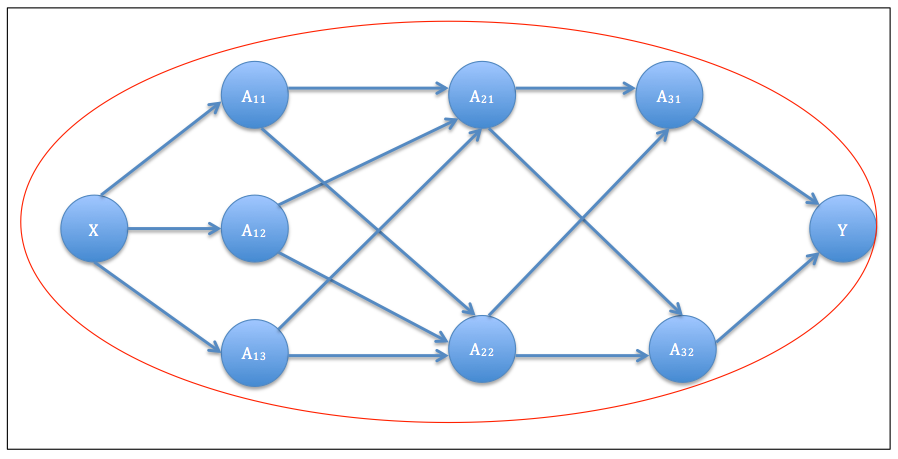
\includegraphics[scale=0.4]{img/EP/CASH}
    \caption{Combined algorithm selection and hyper-parameter optimization in a data analytic pipeline. The algorithms and corresponding hyper-parameters are optimized simultaneously.}
    \label{fig:CASH}
\end{figure}
The second framework is the hyperparameter optimization (HPO) framework where each path in the pipeline is optimized individually. This is described in detail in section \ref{subsubsec_HPO}. This framework is used for quantifying the contribution and propagation of error with respect to \textit{algorithms} in the each path of the pipeline.
\begin{figure}[ht!]
    \centering
    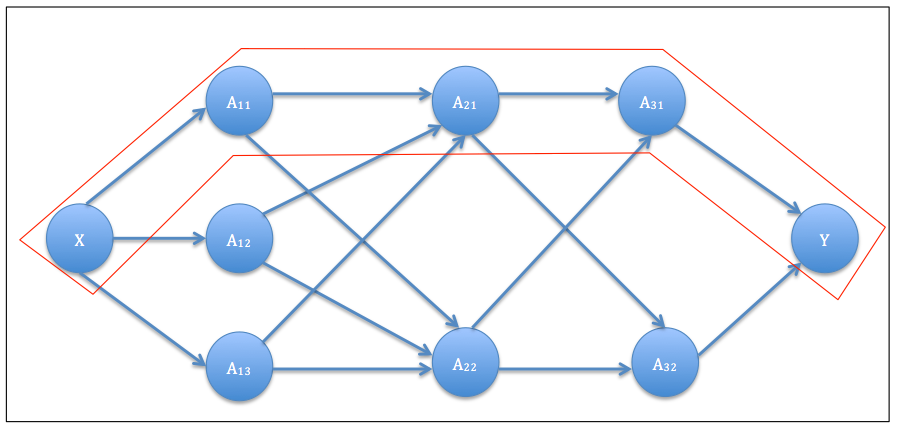
\includegraphics[scale=0.4]{img/EP/HPO}
    \caption{Hyper-parameter optimization in a data analytic pipeline. Each path in the pipeline is individually optimized.}
    \label{fig:HPO}
\end{figure}
Specifically, we choose the path \textit{haralick texture features} - \textit{PCA} - \textit{random forests} to demonstrate the error quantification approach for algorithms.

\subsection{Datasets}
Four datasets from the domains of medicine and material science are used in this work. They are image datasets of breast cancer\cite{bilgin2007cell}, brain cancer \cite{gunduz2004cell}, and two datasets of microstructures in material science \cite{chowdhury2016image}. They are described in the following table.

\begin{table}[ht!]
\centering
\caption{Notations for error definitions used in the error propagation model}
\begin{tabular}{ |c|c| } 
 \hline
 Dataset (notation) & Distribution of classes \\ 
 \hline
 Breast cancer (\textit{breast}) \cite{bilgin2007cell} & \textit{benign}: 151, \textit{in-situ}: 93, \textit{invasive}: 202\\
 \hline
 Brain cancer (\textit{brain}) \cite{gunduz2004cell} & \textit{glioma}: 16, \textit{healthy}: 210, \textit{inflammation}: 107\\
 \hline
  Material science 1 (\textit{matsc1}) \cite{chowdhury2016image} & \textit{dendrites}: 441, \textit{non-dendrites}: 132 \\
 \hline
 Material science 2 (\textit{matsc2}) \cite{chowdhury2016image} & \textit{transverse}: 393, \textit{longitudinal}: 48 \\
 \hline
 \end{tabular}
\label{table:datasets}
\end{table}
The above table represents datasets from the scientific domain. These datasets have been chosen because they represent examples of real world datasets. They are noisy in the sense that they have artefacts in the images, are heavily imbalanced and are small in terms of number of samples. They are different from the very large datasets like ImageNet \cite{deng2009imagenet}, where deep learning techniques like convolutional neural networks have been shown to be superior. Even though deep neural networks represent an end-to-end workflow where the input image is fed into the network and the output classification is obtained at the other end, they may also be represented as pipelines, if the hyper-parameters of the network are considered. \cite{shin2016deep} has shown that machine learning problems involving datasets from medical imaging may be solved using pre-trained and fine-tuned neural networks rather than training them from scratch. We have therefore used pre-trained models such as VGGnet \cite{simonyan2014very} and InceptionNet \cite{szegedy2016rethinking} as pre-trained feature extraction models that fit naturally in the pipeline framework described here for the purpose of illustrating the error quantification methodology.

\subsection{Error quantification experiments}
\label{eq_expts}
Experiments based on the quantification of error contributions framework described in section \ref{EQ} are presented here. The plots are of the error contribution values calculated using Eqs. \ref{eq_step}, \ref{eq_alg} \ref{fig:eq_hyper} on the 4 datasets described in Table 3. The error contribution values are obtained from the trials in the optimization methods described in Section \ref{sec2}. Grid search is only run once while the other algorithms are averaged over 5 runs with the mean and standard deviation shown in the following plots. These results are computed on the validation error (cross-entropy loss) obtained at the end of the pipeline. Random search and Bayesian optimization (using the SMAC algorithm) are implemented on both the frameworks described in Section \ref{frameworks} for computational steps and algorithms respectively. The grid search results maybe used as the gold standard to compare the performance of other optimization algorithms. 

\subsubsection{Error contribution from computational steps}
The mean and standard deviation values of $EC_{S_i}$ calculated using Eq. \ref{eq_step} is represented in Fig. \ref{fig:eq_steps} for the 4 datasets in Table \ref{table:datasets}. The error is calculated using the formulation of $EC_{S_i}$ in section \ref{subsubsec_eq_steps}. We can observe that most of the contribution comes from feature extraction algorithms. This means that it is most important to optimize the feature extraction step among the other steps as it is of most importance based on the plots. This confirms our intuitive belief that feature extraction algorithms are the most important components of a machine learning pipeline. 
\begin{figure}[ht!]
\centering
\begin{subfigure}{.5\textwidth}
  \centering
  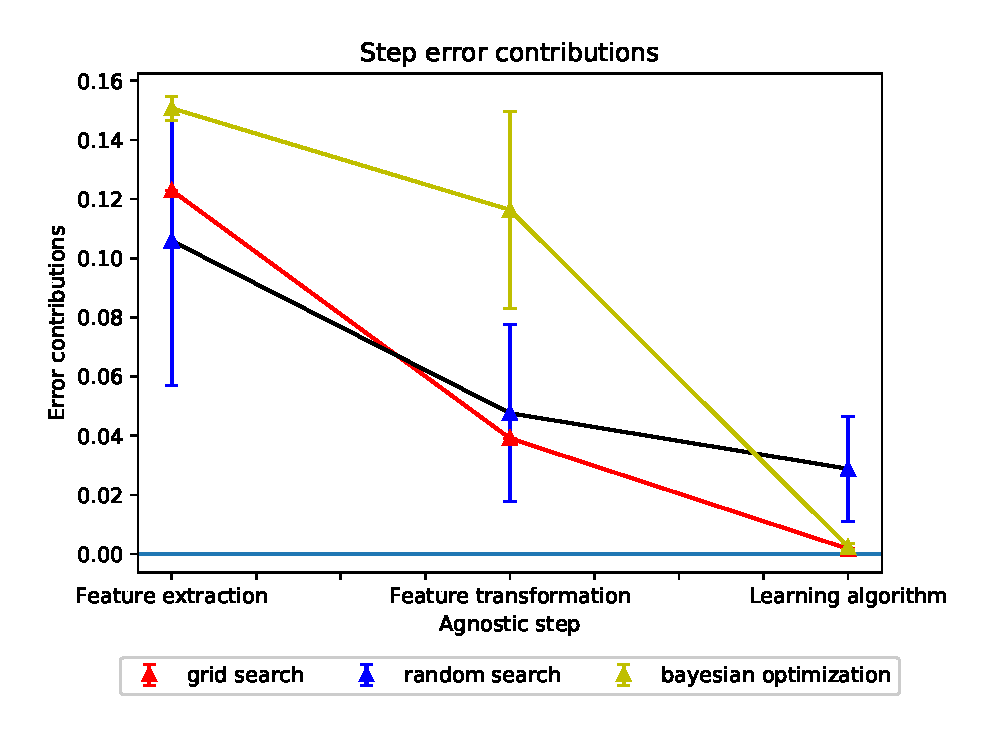
\includegraphics[scale=0.37]{img/EP/agnostic_error_steps_breast}
  \caption{\textit{breast}}
  \label{fig:eq_steps_breast}
\end{subfigure}%
\begin{subfigure}{.5\textwidth}
  \centering
  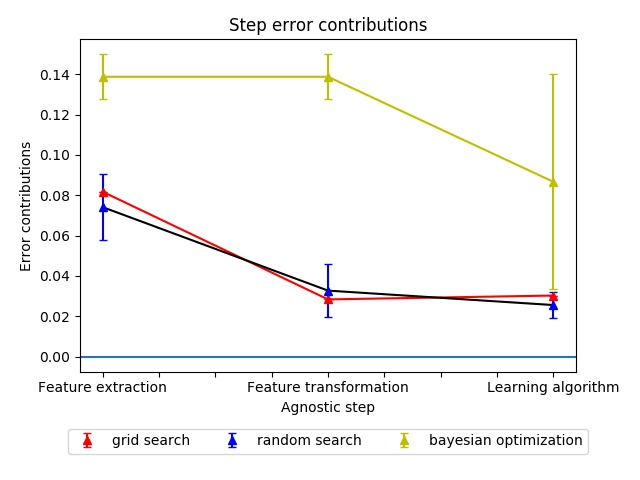
\includegraphics[scale=0.37]{img/EP/agnostic_error_step_brain}
  \caption{\textit{brain}}
  \label{fig:eq_step_brain}
\end{subfigure}
\begin{subfigure}{.5\textwidth}
  \centering
  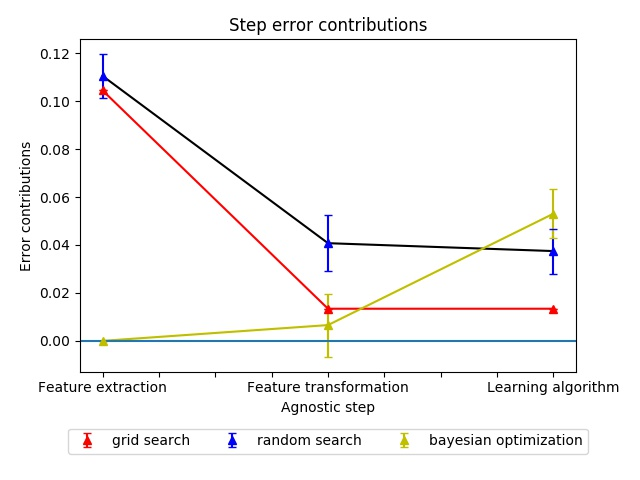
\includegraphics[scale=0.37]{img/EP/agnostic_error_step_matsc_dataset1}
  \caption{\textit{matsc1}}
  \label{fig:eq_steps_matsc1}
\end{subfigure}%
\begin{subfigure}{.5\textwidth}
  \centering
  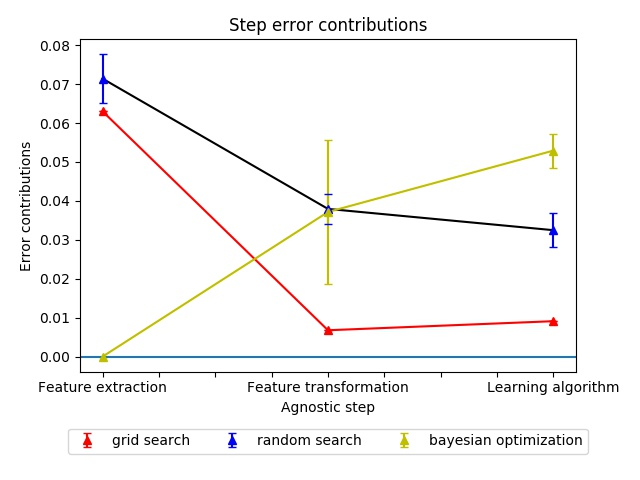
\includegraphics[scale=0.37]{img/EP/agnostic_error_step_matsc_dataset2}
  \caption{\textit{matsc2}}
  \label{fig:eq_steps_matsc2}
\end{subfigure}
\caption{Plots of error contributions from computational steps in the pipeline. Random search (blue) follows the behavior of grid search (red), whereas, bayesian optimization does not. Hence, random search maybe used to quantify the error contributions instead of grid search.}
\label{fig:eq_steps}
\end{figure}

 The standard deviation of grid search is 0 because it was only run once for each dataset due to the time required for computation and also because of the robustness of the grid search method (the results don't change because we try out every single configuration). We observe from the results, that random search follows the behavior of grid search. It mirrors the behavior of grid search, but the results are not robust because of the high standard deviation. This is expected because the search trials may not include all the configurations of algorithms in the pipeline as opposed to grid search where all the configurations of algorithms and hyperparameters are evaluated. The results of SMAC (bayesian optimization) in the CASH framework do not follow the behavior of grid search. This is because the trials for SMAC are even more sparse with respect to the algorithms it selects for optimization of  the error in Eq. \ref{eq_step}. SMAC only samples a few configurations based on the updated probabilistic model as it narrows in on the optimum error. Therefore, it sometimes gives erroneous results as can be seen for $matsc1$ and $matsc2$ in Figs. \ref{fig:eq_steps_matsc1} and \ref{fig:eq_steps_matsc2} respectively.


\subsubsection{Error contribution from algorithms}

% In the following figure, the error contributions from algorithms are quantified using theformulation in Section 3.1.2.  This is represented asmethod1 in the experiments.  As men-tioned before, we see that only 3 algorithms corresponding to the each step in the pipelinethat lie on the best path are dominant in terms of error contribution.
In the following figure, the error contributions from algorithms are quantified using the formulation in Section \ref{subsubsec_eq_alg}. We select \textit{haralick texture features}, $PCA$ and \textit{random forests} as the path to demonstrate the contribution of error from algorithms, because each of these algorithms are associated with one or more hyper-parameters. We observe a trend here, in that, the error contributed from \textit{haralick texture features} and \textit{random forests} is more than $PCA$. This means that it is more important to tune \textit{haralick texture features}, and \textit{random forests} than it is to tune  $PCA$. Again, we see the trend that random search performs better in terms of following the behavior of grid search than Bayesian optimization.

% This issue is redressed by the second  formulation for error contribution from algorithms in 3.1.2 which is shown in Fig. 9.
\begin{figure}[ht!]
\centering
\begin{subfigure}{.5\textwidth}
  \centering
  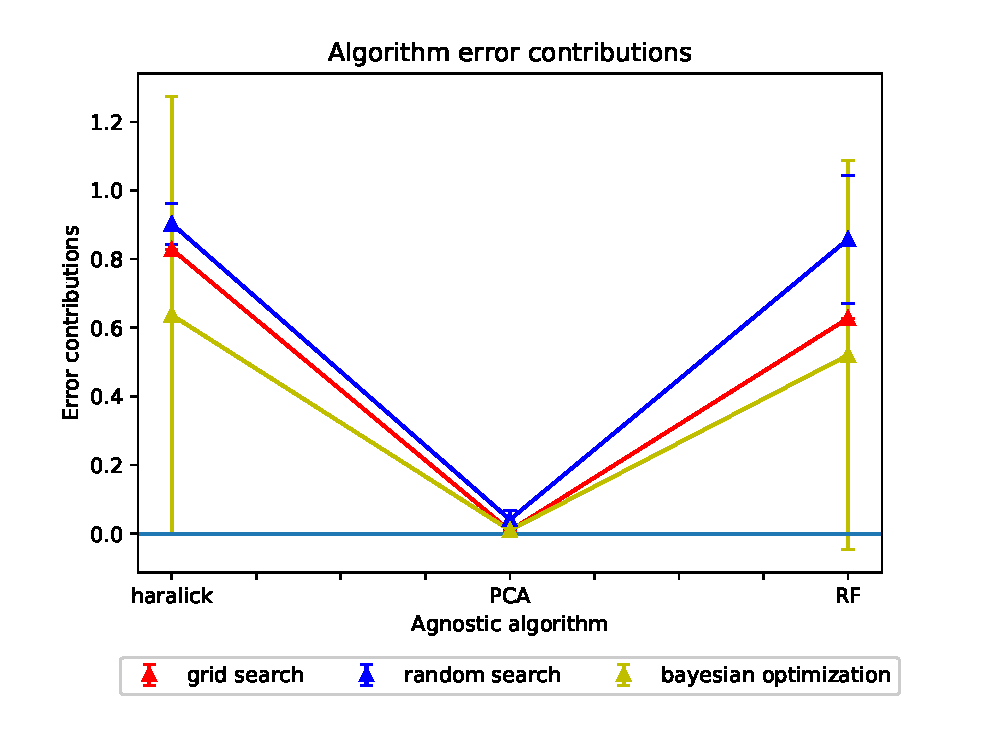
\includegraphics[scale=0.37]{img/EP/agnostic_error_alg_breast}
  \caption{\textit{breast}}
  \label{fig:sfig1}
\end{subfigure}%
\begin{subfigure}{.5\textwidth}
  \centering
  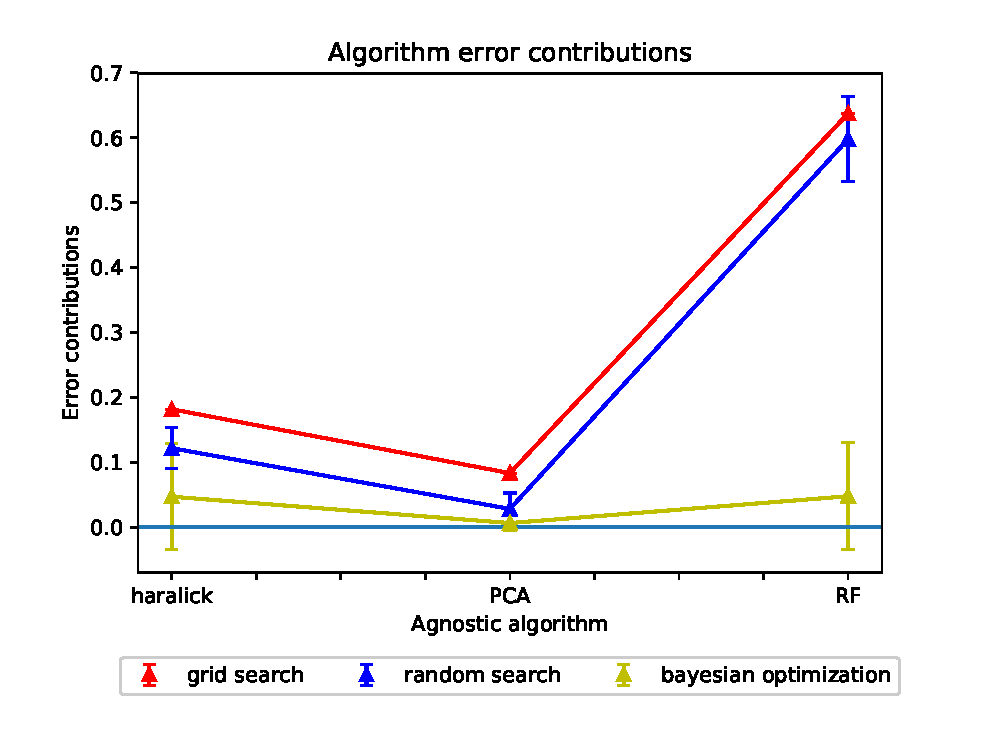
\includegraphics[scale=0.37]{img/EP/agnostic_error_alg_brain}
  \caption{\textit{brain}}
  \label{fig:sfig2}
\end{subfigure}
\begin{subfigure}{.5\textwidth}
  \centering
  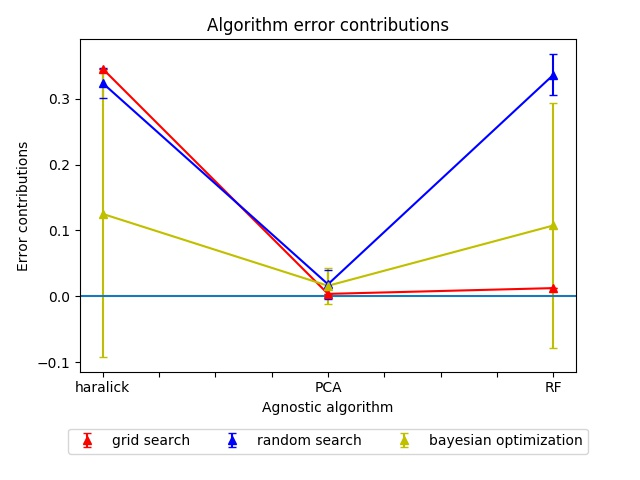
\includegraphics[scale=0.37]{img/EP/agnostic_error_alg_matsc_dataset1}
  \caption{\textit{matsc1}}
  \label{fig:sfig3}
\end{subfigure}%
\begin{subfigure}{.5\textwidth}
  \centering
  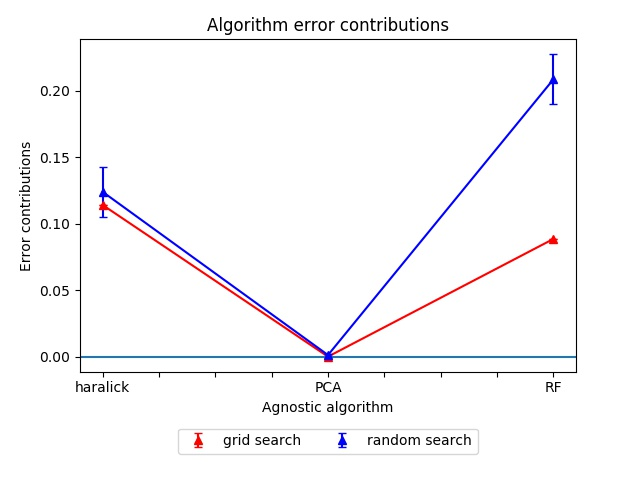
\includegraphics[scale=0.37]{img/EP/agnostic_error_alg_matsc_dataset2}
  \caption{\textit{matsc2}}
  \label{fig:sfig4}
\end{subfigure}

\caption{Plots of error contributions from algorithms in the pipeline. Random search again mirrors the trend of grid search more than bayesian optimization. Therefore random search maybe used instead of grid search for computing the contribution of error from algorithms in a path. The plots also show that it is more important to tune \textit{haralick texture features}, and \textit{random forests} than it is to tune  $PCA$. }
\label{fig:fig}
\end{figure}

\subsubsection{Error contribution from hyper-parameters}

% In the following figure, the error contributions from algorithms are quantified using theformulation in Section 3.1.2.  This is represented asmethod1 in the experiments.  As men-tioned before, we see that only 3 algorithms corresponding to the each step in the pipelinethat lie on the best path are dominant in terms of error contribution.
Fig. \ref{fig:eq_hyper} shows the error contributions from hyper-parameters quantified using the formulation in Section \ref{subsubsec_eq_hyper}. We again select \textit{haralick texture features}, $PCA$ and \textit{random forests} as the path to demonstrate the contribution of error from algorithms. Again, we see the trend that random search performs better in terms of following the behavior of grid search than Bayesian optimization. In addition, we observe that it is in general more important to tune the hyper-parameters \textit{Haralick distance}, and \textit{Number of estimators} than it is to tune  the other hyper-parameters.

% This issue is redressed by the second  formulation for error contribution from algorithms in 3.1.2 which is shown in Fig. 9.
\begin{figure}[ht!]
\centering
\begin{subfigure}{.5\textwidth}
  \centering
  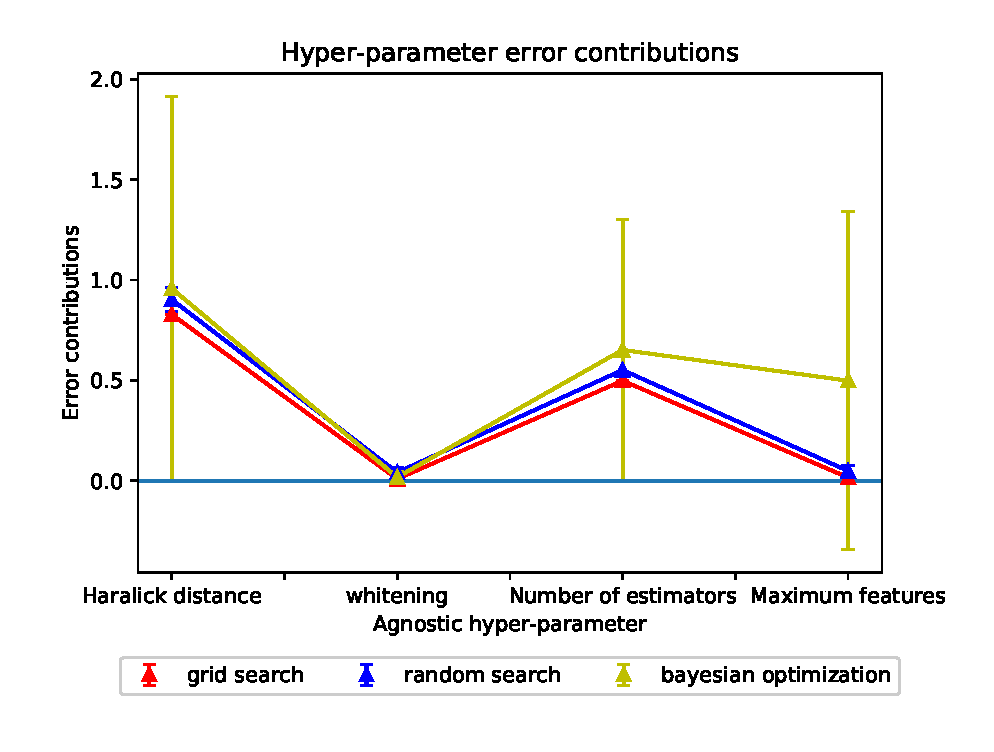
\includegraphics[scale=0.37]{img/EP/agnostic_error_hyper_breast}
  \caption{\textit{breast}}
  \label{fig:sfig1}
\end{subfigure}%
\begin{subfigure}{.5\textwidth}
  \centering
  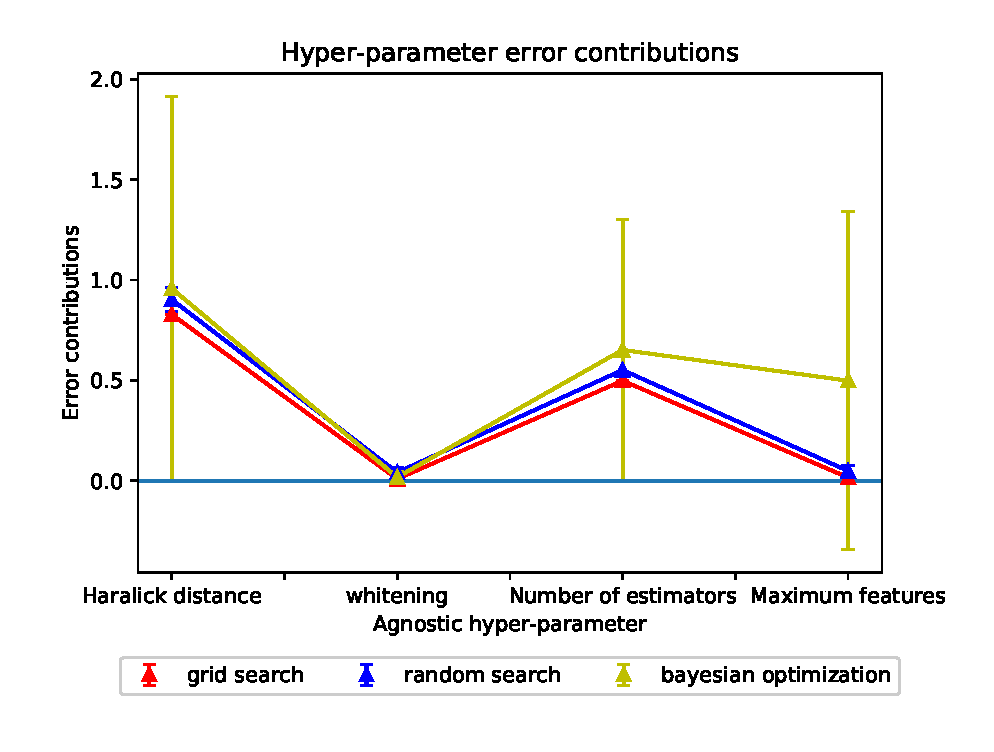
\includegraphics[scale=0.37]{img/EP/agnostic_error_hyper_breast}
  \caption{\textit{brain}}
  \label{fig:sfig2}
\end{subfigure}
\begin{subfigure}{.5\textwidth}
  \centering
  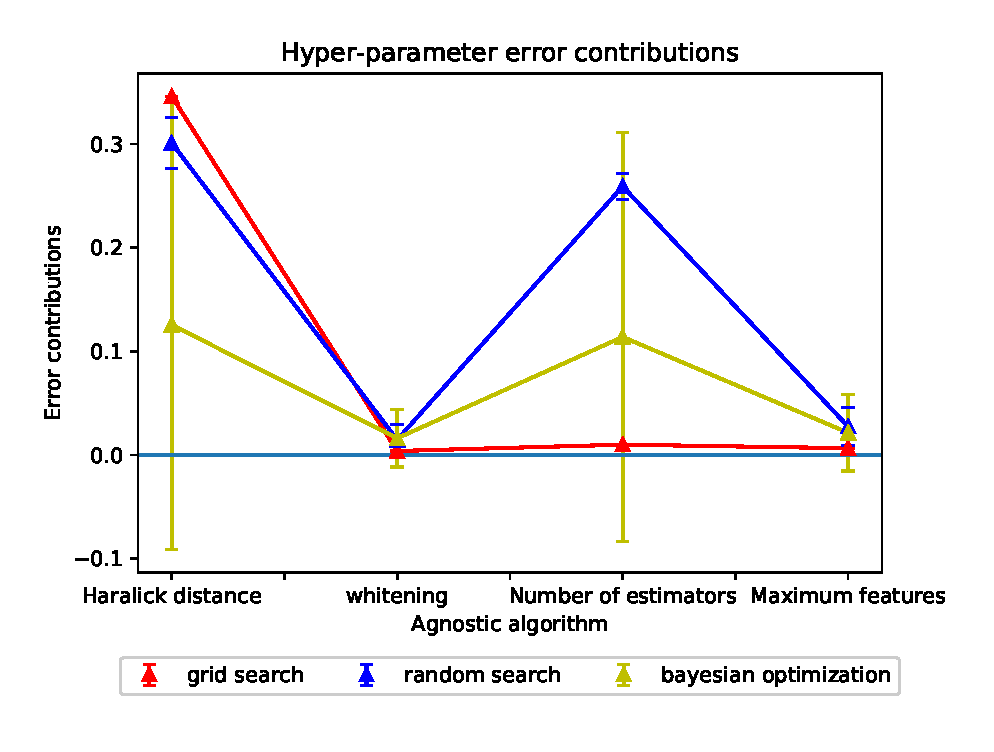
\includegraphics[scale=0.37]{img/EP/agnostic_error_hyper_matsc_dataset1}
  \caption{\textit{matsc1}}
  \label{fig:sfig3}
\end{subfigure}%
\begin{subfigure}{.5\textwidth}
  \centering
  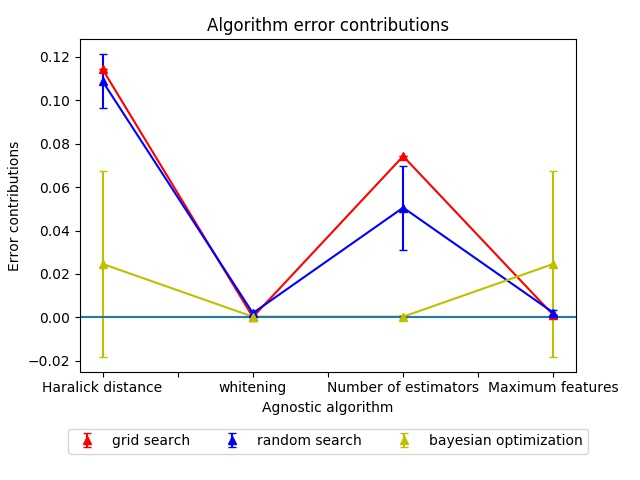
\includegraphics[scale=0.37]{img/EP/agnostic_error_hyper_matsc_dataset2}
  \caption{\textit{matsc2}}
  \label{fig:sfig4}
\end{subfigure}

\caption{Plots of error contributions from hyper-parameters in the pipeline. Random search again mirrors the trend of grid search more than bayesian optimization. Therefore random search maybe used instead of grid search for computing the contribution of error from hyper-parameters in a path. The plots also show that it is more important to tune the hyper-parameters \textit{Haralick distance}, and \textit{Number of estimators} than it is to tune  the other hyper-parameters.}
\label{fig:eq_hyper}
\end{figure}



% As expected, in each of the above figures, we observe that 3 algorithms stand out for each of the datasets. This formulation gives us an idea as to which algorithms are important in terms of their contribution to the final optimized validation error. In other words, the combination of these 3 algorithms are in the optimal path when the pipelines are run for the 4 datasets. 
% Similar to the results from Fig. 7, we also observe that the HPO formulations provide more accurate results than their CASH counterparts. In addition, for reasons explained above, the bayesian optimization on the CASH framework is more erroneous than the random search results.

% The experiments in the following figure correspond to the second formulation given by Eq. \ref{eq_alg2} in Section 3.1.2. As can be seen from the following results, this provides a better representation of error contribution from the algorithms and not just 3 dominant algorithms in Fig 8.

% \begin{figure}[H]
% \centering
% \begin{subfigure}{.5\textwidth}
%   \centering
%   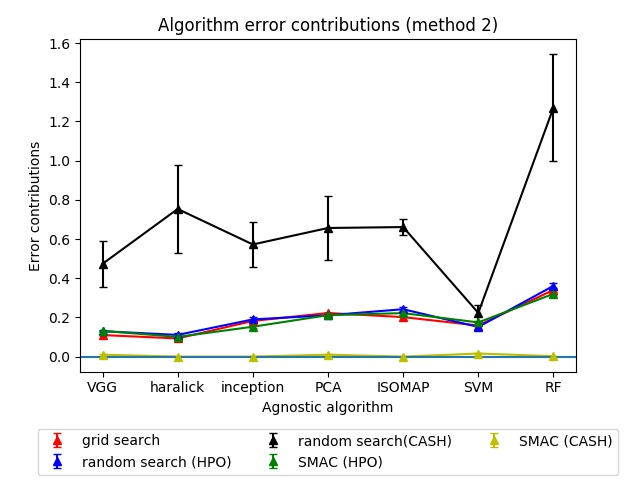
\includegraphics[scale=0.37]{agnostic_error_alg_2_breast}
%   \caption{\textit{breast}}
%   \label{fig:sfig1}
% \end{subfigure}%
% \begin{subfigure}{.5\textwidth}
%   \centering
%   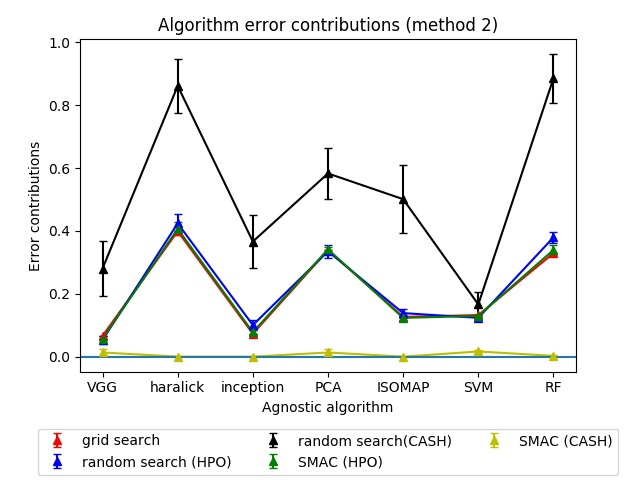
\includegraphics[scale=0.37]{agnostic_error_alg_2_brain}
%   \caption{\textit{brain}}
%   \label{fig:sfig2}
% \end{subfigure}
% \begin{subfigure}{.5\textwidth}
%   \centering
%   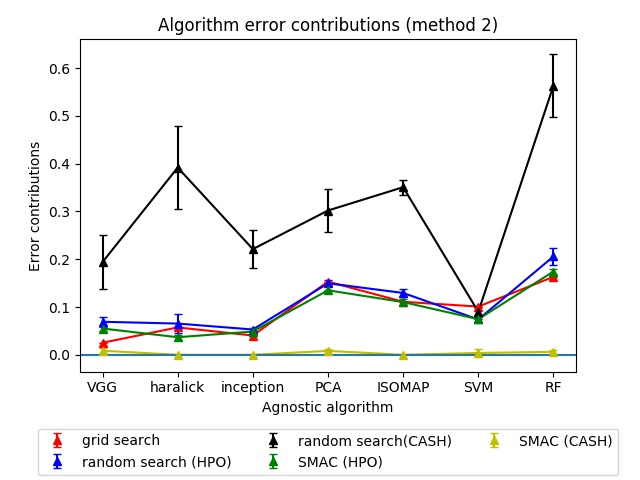
\includegraphics[scale=0.37]{agnostic_error_alg_2_matsc_dataset1}
%   \caption{\textit{matsc1}}
%   \label{fig:sfig3}
% \end{subfigure}%
% \begin{subfigure}{.5\textwidth}
%   \centering
%   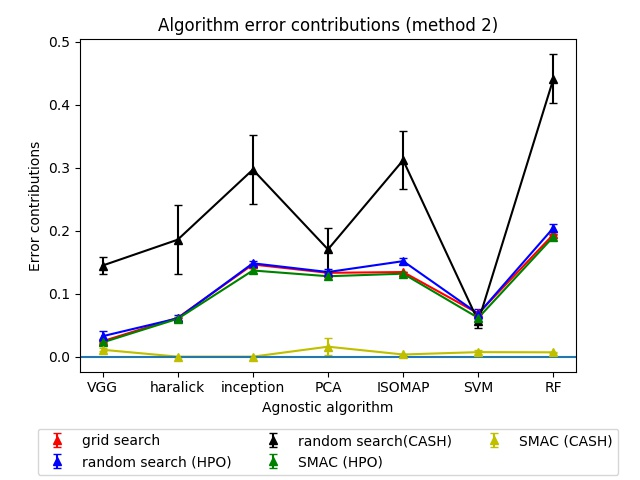
\includegraphics[scale=0.37]{agnostic_error_alg_2_matsc_dataset2}
%   \caption{\textit{matsc2}}
%   \label{fig:sfig4}
% \end{subfigure}

% \caption{Plots of error contributions from algorithms in the pipeline (method 2).}
% \label{fig:fig}
% \end{figure}
% We can see from the plots in the figure above that the error is distributed among various algorithms and not just 3 dominant algorithms. This error can be regarded as the cost of not optimizing the path that flows through the particular algorithm.
% We again observe the same trend while comparing the different optimization approaches. HPO does a better job at capturing the error contribution for reasons stated above. Random search in the CASH framework follows the behavior of grid search but has higher variance. SMAC does a poor job at computing the error contributions from the pipeline altogether. 

\subsubsection{Comparison of computation time}
Fig. \ref{fig:time} shows the average computation times of each of the algorithms used in the error quantification experiments. We can observe that random search and bayesian optimization are both efficient in terms of computational time as opposed to grid search. As expected, the CASH based optimization runs faster than the corresponding HPO counterparts.
Therefore, both CASH and HPO optimization frameworks using algorithms like Random search and Bayesian optimization maybe used for computation of the error contributions instead of grid search. However, as we have seen repeatedly from the plots in Figs. \ref{fig:eq_steps}, \ref{fig:eq_alg} and \ref{fig:eq_hyper}; random search captures the behavior of grid search more accurately. Hence, random search maybe used to quantify the contributions from steps, algorithms and hyper-parameters accurately and efficiently.

\begin{figure}[H]
    \centering
    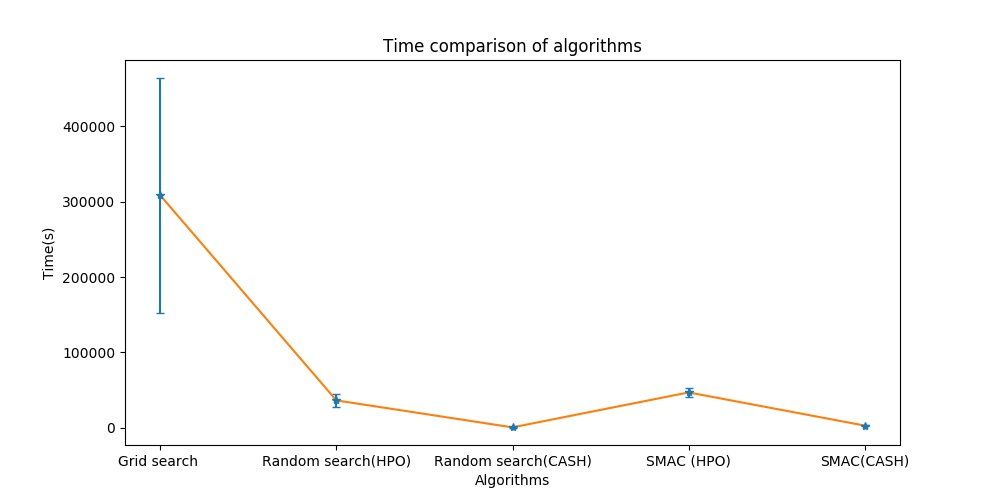
\includegraphics[scale=0.4]{img/EP/times_algorithms}
    \caption{Pipeline including naive algorithms for error propagation. Random search and bayesian optimization are both much more efficient that grid search in terms of computation time.}
    \label{fig:time}
\end{figure}



% \subsection{Error propagation experiments}
% The set of experiments in this section correspond to the error propagation model formulated in Section 3.2. The corresponding pipeline including the naive algorithms are represented in the following figure.

% \begin{figure}[H]
%     \centering
%     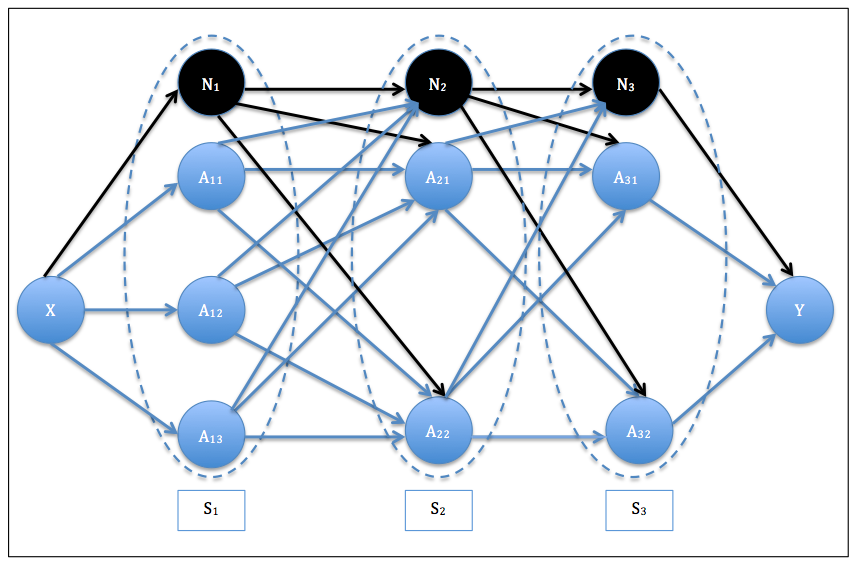
\includegraphics[scale=0.5]{naive}
%     \caption{Pipeline including naive algorithms for error propagation}
%     \label{fig:flowchart}
% \end{figure}

% The naive algorithms used in this work are \textit{vectorization} (flattening the image into a vector) for feature extraction, \textit{no transformation} for feature transformation, and \textit{1-nearest neaighbors} algorithm as the classification or learning algorithm. The naive algorithms are selected with the assumption that the only error that result from them is the direct error, as discussed in Section 3.2.

% The following figures shows the results of the error propagation framework. The results are obtained based on the CASH based random search for steps and HPO based random search on paths for algorithms. 
% Fig. 11 shows the plots for error propagation along the steps in the image classification pipeline. The plots show the total error $EC_{S_i}$, the direct error $E_{direct}$ and the propagation error $E_{propagation}$. These values are computed using error propagation model defined in section 3.2.1.
% The total error is the error contribution calculated using Eq. 3. We can see from the results that the total error is dominated by the direct error from the algorithms in the steps. The propagation error is the difference between the total error and the direct error from the algorithms. We also note that the propagation error progressively reduces in magnitude from feature extraction algorithms (that are at the beginning of the pipeline) to learning algorithms (that are at the end of the pipeline). Therefore, the model captures our intuition that usually more error is propagated from steps that exist closer to the beginning of the pipeline.

% \begin{figure}[H]
% \centering
% \begin{subfigure}{.5\textwidth}
%   \centering
%   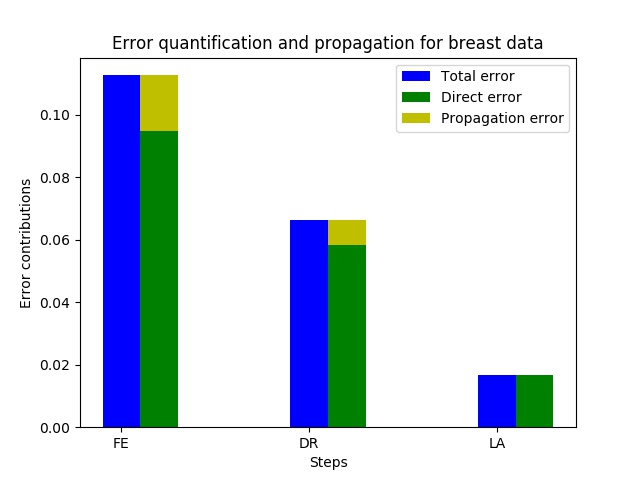
\includegraphics[scale=0.4]{error_propagation_random_pipeline_breast}
%   \caption{\textit{breast}}
%   \label{fig:sfig1}
% \end{subfigure}%
% \begin{subfigure}{.5\textwidth}
%   \centering
%   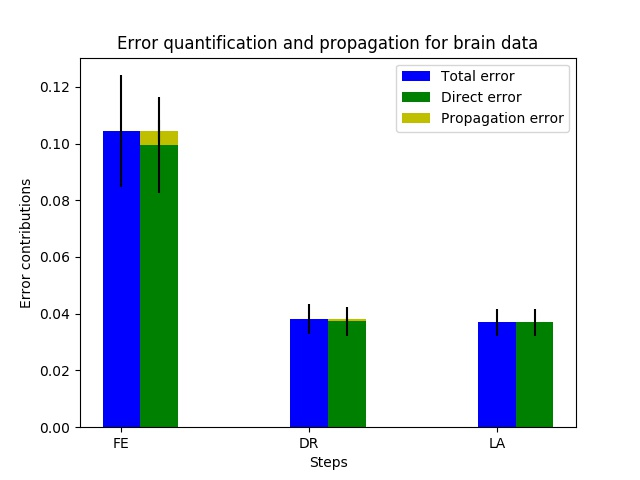
\includegraphics[scale=0.4]{error_propagation_random_pipeline_brain}
%   \caption{\textit{brain}}
%   \label{fig:sfig2}
% \end{subfigure}
% \begin{subfigure}{.5\textwidth}
%   \centering
%   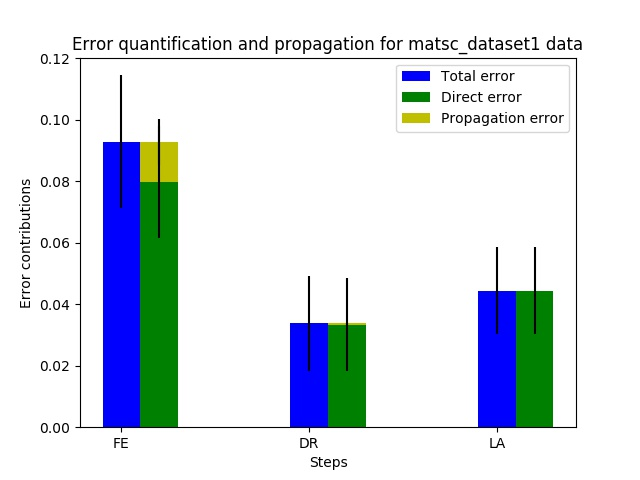
\includegraphics[scale=0.4]{error_propagation_random_pipeline_matsc_dataset1}
%   \caption{\textit{matsc1}}
%   \label{fig:sfig3}
% \end{subfigure}%
% \begin{subfigure}{.5\textwidth}
%   \centering
%   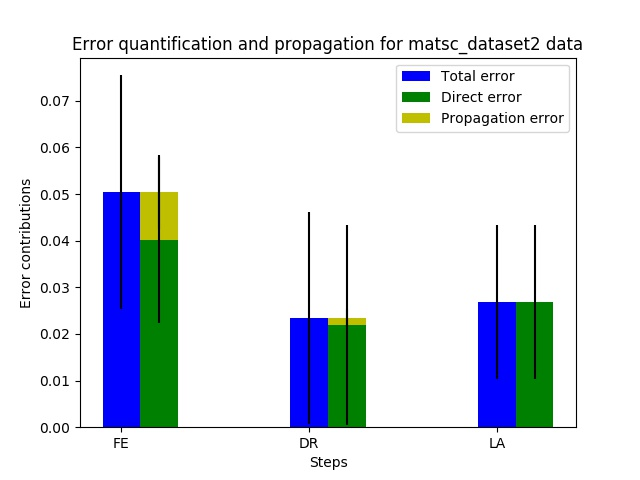
\includegraphics[scale=0.4]{error_propagation_random_pipeline_matsc_dataset2}
%   \caption{\textit{matsc2}}
%   \label{fig:sfig4}
% \end{subfigure}

% \caption{Plots of error propagation using the naive algorithm based methodology. The total error is dominated by the direct error introduced by the steps. The propagation error reduces as we move toward the end of the pipeline.}
% \label{fig:fig}
% \end{figure}

% The following figure shows the propagation factor $\gamma$ computed in Eq. 6. The value of this factor quantifies the propagation from a particular step in the pipeline. A relatively high value means that the factor by which the error is propagated down the pipeline from a particular step is large. As expected, we observe that the propagation factors are large for feature extraction algorithms and they progressively reduce in magnitude as we move closer towards the end of the pipeline. The propagation factor for learning algorithms is $0$ because this step is at the end of the pipeline, and all the error from the step is directly due to the algorithms themselves and no error is propagated.

% \begin{figure}[H]
% \centering
% \begin{subfigure}{.5\textwidth}
%   \centering
%   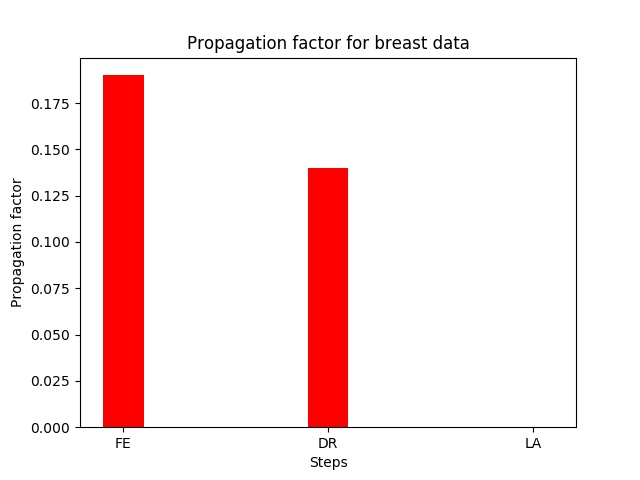
\includegraphics[scale=0.4]{propagation_factor_random_pipeline_breast}
%   \caption{\textit{breast}}
%   \label{fig:sfig1}
% \end{subfigure}%
% \begin{subfigure}{.5\textwidth}
%   \centering
%   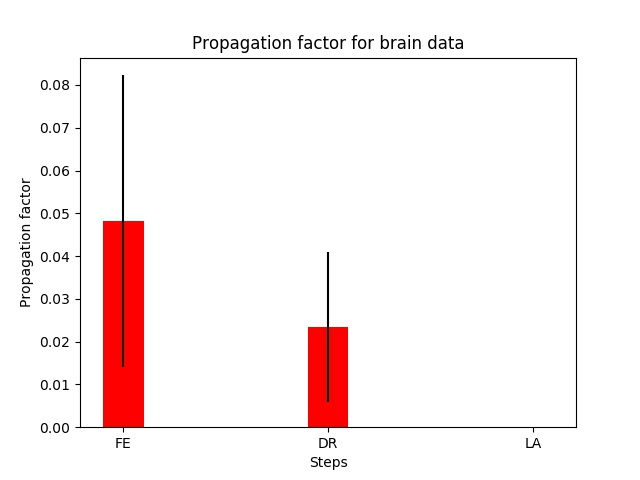
\includegraphics[scale=0.4]{propagation_factor_random_pipeline_brain}
%   \caption{\textit{brain}}
%   \label{fig:sfig2}
% \end{subfigure}
% \begin{subfigure}{.5\textwidth}
%   \centering
%   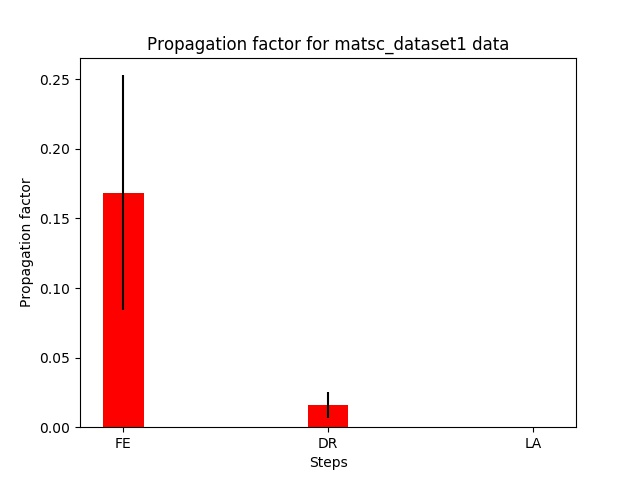
\includegraphics[scale=0.4]{propagation_factor_random_pipeline_matsc_dataset1}
%   \caption{\textit{matsc1}}
%   \label{fig:sfig3}
% \end{subfigure}%
% \begin{subfigure}{.5\textwidth}
%   \centering
%   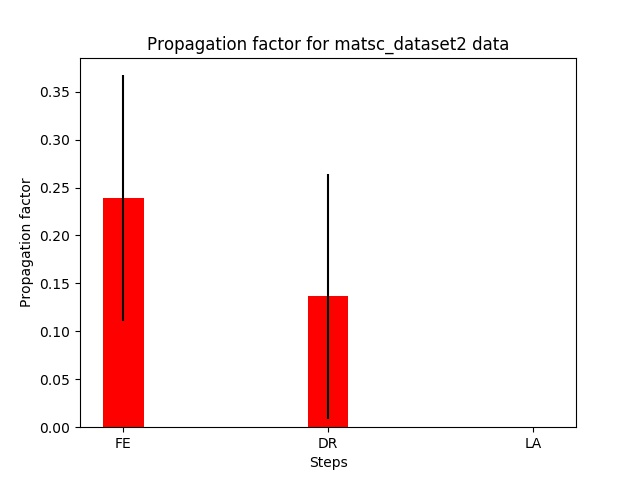
\includegraphics[scale=0.4]{propagation_factor_random_pipeline_matsc_dataset2}
%   \caption{\textit{matsc2}}
%   \label{fig:sfig4}
% \end{subfigure}

% \caption{Plots of propagation factor $\gamma$ using the naive algorithm based methodology. The propagation factors are higher for steps closer to the beginning of the pipeline and progressively reduce in magnitude towards the end of the pipeline. The propagation factor from learning algorithms is non-existent because no error is propagated.}
% \label{fig:fig}
% \end{figure}

% The same computations for error propagation are carried out with respect to algorithms. Again in this formulation, we optimize a path in the pipeline. The path used here is the same as that used in the error contribution experiments for algorithms in section 4.3.2 - \textit{haralick texture features}, $PCA$ and \textit{random forests}. The following figures represent the corresponding plots representing the error propagation and propagation factors with respect to algorithms.

% \begin{figure}[H]
% \centering
% \begin{subfigure}{.5\textwidth}
%   \centering
%   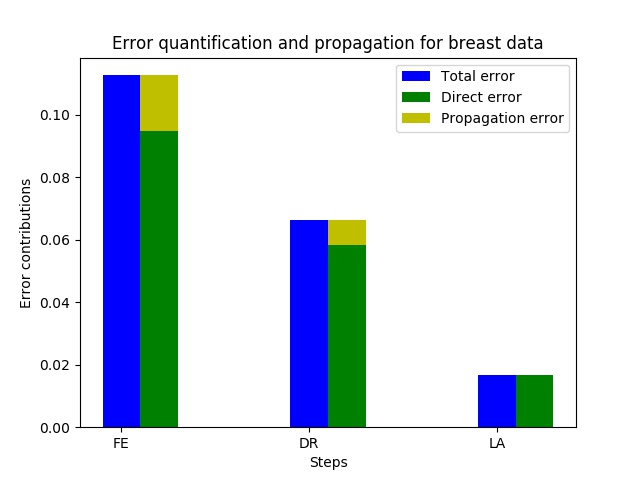
\includegraphics[scale=0.4]{error_propagation_random_pipeline_breast}
%   \caption{\textit{breast}}
%   \label{fig:sfig1}
% \end{subfigure}%
% \begin{subfigure}{.5\textwidth}
%   \centering
%   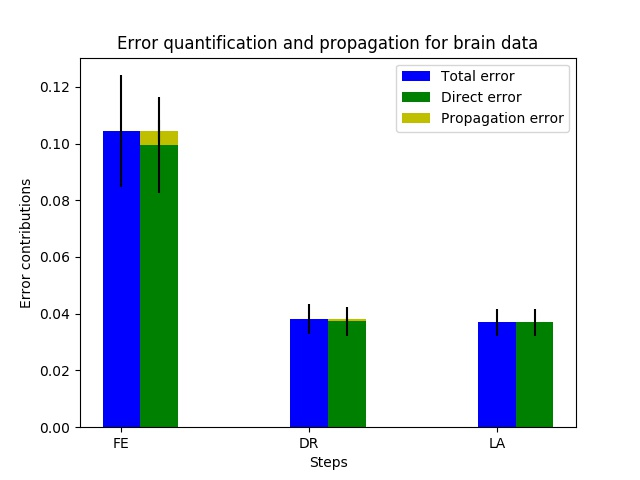
\includegraphics[scale=0.4]{error_propagation_random_pipeline_brain}
%   \caption{\textit{brain}}
%   \label{fig:sfig2}
% \end{subfigure}
% \begin{subfigure}{.5\textwidth}
%   \centering
%   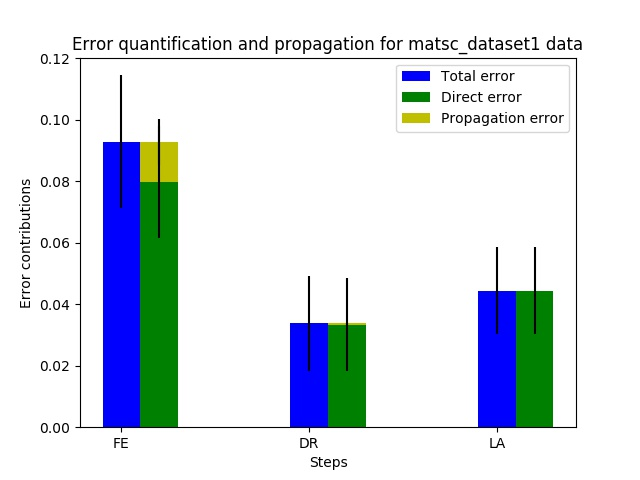
\includegraphics[scale=0.4]{error_propagation_random_pipeline_matsc_dataset1}
%   \caption{\textit{matsc1}}
%   \label{fig:sfig3}
% \end{subfigure}%
% \begin{subfigure}{.5\textwidth}
%   \centering
%   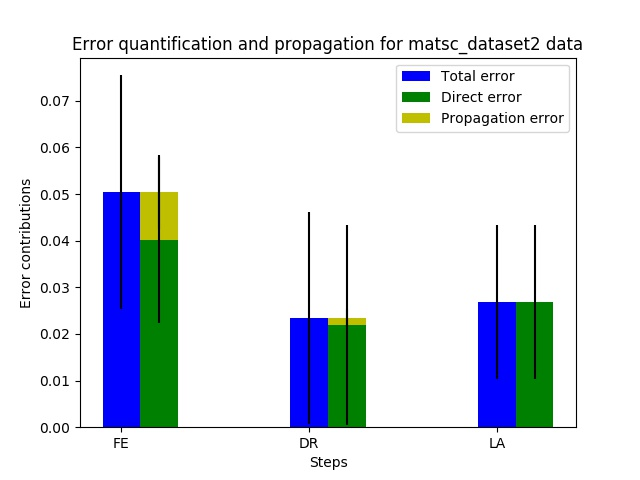
\includegraphics[scale=0.4]{error_propagation_random_pipeline_matsc_dataset2}
%   \caption{\textit{matsc2}}
%   \label{fig:sfig4}
% \end{subfigure}

% \caption{Plots of error propagation from the steps using the naive algorithm based methodology.}
% \label{fig:fig}
% \end{figure}


% \begin{figure}[H]
% \centering
% \begin{subfigure}{.5\textwidth}
%   \centering
%   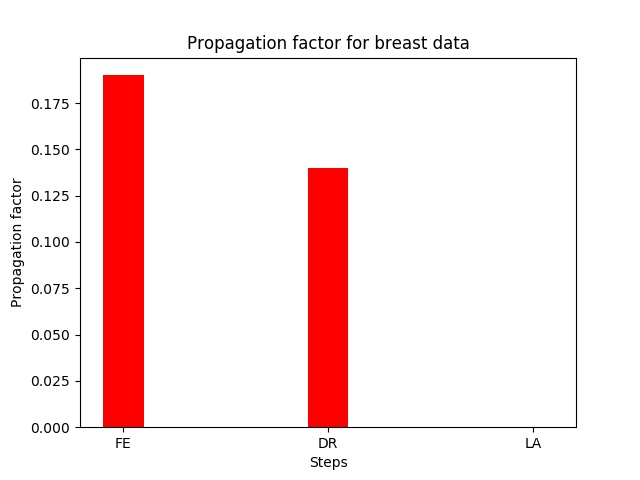
\includegraphics[scale=0.4]{propagation_factor_random_pipeline_breast}
%   \caption{\textit{breast}}
%   \label{fig:sfig1}
% \end{subfigure}%
% \begin{subfigure}{.5\textwidth}
%   \centering
%   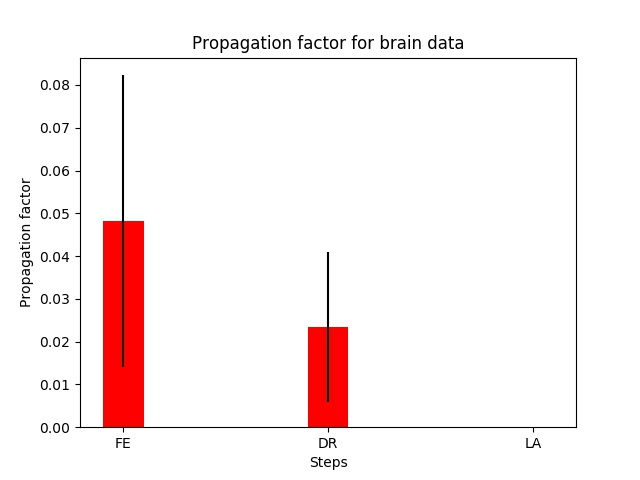
\includegraphics[scale=0.4]{propagation_factor_random_pipeline_brain}
%   \caption{\textit{brain}}
%   \label{fig:sfig2}
% \end{subfigure}
% \begin{subfigure}{.5\textwidth}
%   \centering
%   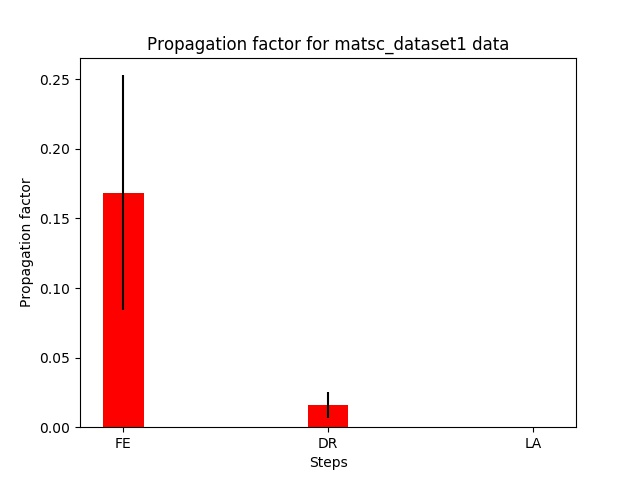
\includegraphics[scale=0.4]{propagation_factor_random_pipeline_matsc_dataset1}
%   \caption{\textit{matsc1}}
%   \label{fig:sfig3}
% \end{subfigure}%
% \begin{subfigure}{.5\textwidth}
%   \centering
%   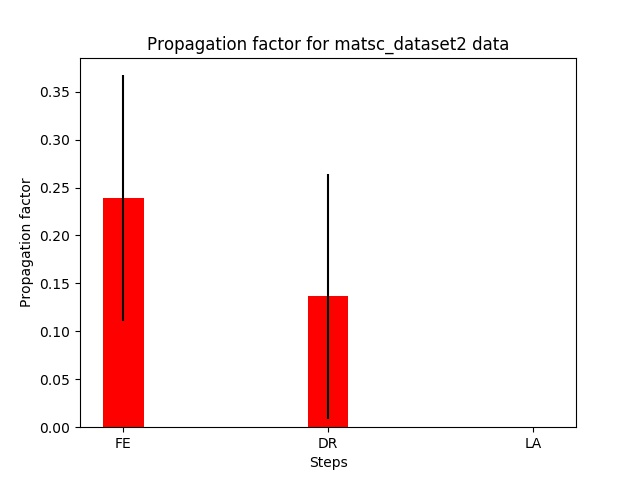
\includegraphics[scale=0.4]{propagation_factor_random_pipeline_matsc_dataset2}
%   \caption{\textit{matsc2}}
%   \label{fig:sfig4}
% \end{subfigure}

% \caption{Plots of propagation factor $\gamma$ from algorithms using the naive algorithm based methodology.}
% \label{fig:fig}
% \end{figure}


% All of the figures shown above are computed with respect to the validation dataset. We also perform the same experiments on the 20 \% held out test data. The following figure shows the results of the error contribution and propagation on the test data for \textit{breast} dataset. We compare the results of the held out test data with the results from the validation data. As we can see, the magnitude of error contributions from the test data are slightly larger that that from validation data. This can be explained due to slight overfitting on the validation dataset. The error propagation results on the test dataset is also different from the validation dataset. This can also be due to error from generalization.

% \begin{figure}[H]
% \centering
% \begin{subfigure}{.5\textwidth}
%   \centering
%   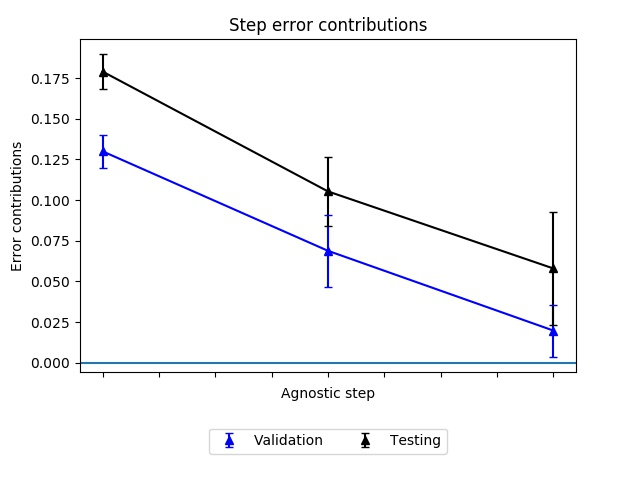
\includegraphics[scale=0.4]{agnostic_error_step_val_test_breast}
%   \caption{\textit{Error contributions from computational steps}}
%   \label{fig:sfig1}
% \end{subfigure}%
% \begin{subfigure}{.5\textwidth}
%   \centering
%   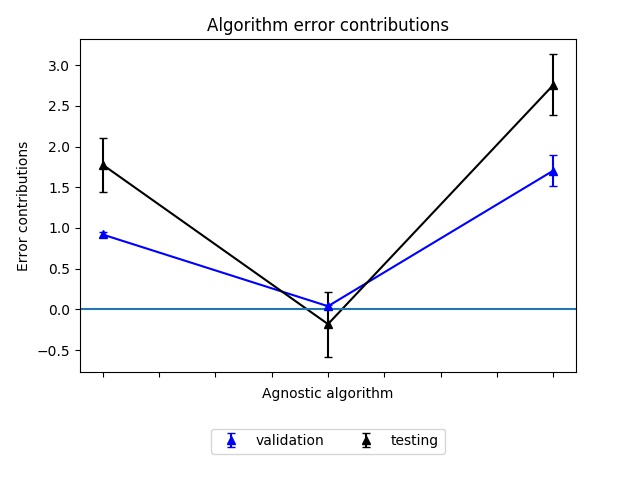
\includegraphics[scale=0.4]{agnostic_error_alg_breast_test}
%   \caption{\textit{Error  from algorithms (\textit{method 1})}}
%   \label{fig:sfig1}
% \end{subfigure}
% % \begin{subfigure}{.5\textwidth}
% %   \centering
% %   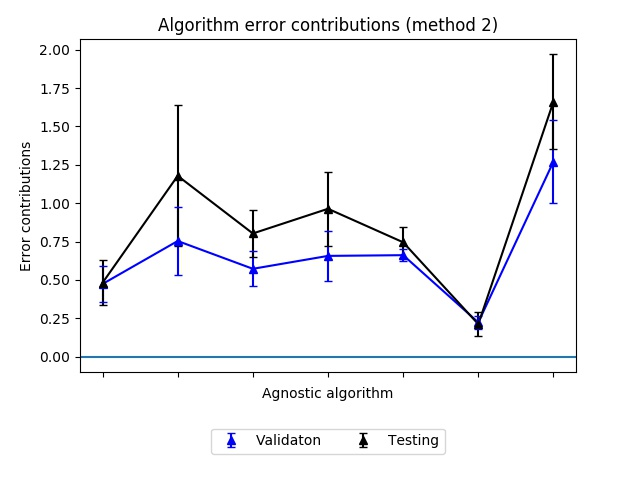
\includegraphics[scale=0.4]{agnostic_error_alg_2_val_test_breast}
% %   \caption{\textit{Error from algorithms (\textit{method 2})}}
% %   \label{fig:sfig1}
% % \end{subfigure}%
% \begin{subfigure}{.5\textwidth}
%   \centering
%   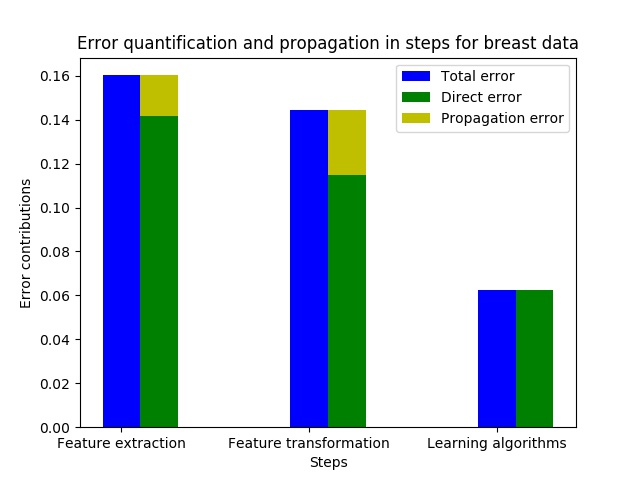
\includegraphics[scale=0.4]{error_propagation_random_pipeline_steps_test_breast}
%   \caption{\textit{Error propagation}}
%   \label{fig:sfig4}
% \end{subfigure}%
% \begin{subfigure}{.5\textwidth}
%   \centering
%   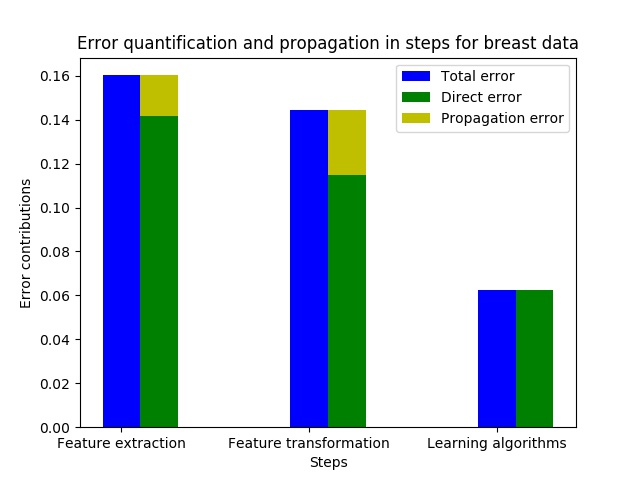
\includegraphics[scale=0.4]{error_propagation_random_pipeline_steps_test_breast}
%   \caption{\textit{Propagation factor}}
%   \label{fig:sfig4}
% \end{subfigure}
% \caption{Plots of error contribution and error propagation on test data from \textit{breast} data. The difference between the results for test and validation data maybe accounted for by the error from generalization.}
% \label{fig:fig}
% \end{figure}


\section{Conclusion}
This work proposes a methodology for making black box machine learning based image classification pipelines interpretable. The suggested approach involves understanding the sources of error in data analytic pipelines. Specifically, we propose a methodology to quantify the error contributions from different parts of an image classification pipeline, namely computational steps, algorithms and hyper-parameters. This methodology is described as the \textit{agnostic} method described in Section \ref{EQ}. The results in Section \ref{eq_expts} show that the black-box optimization methods like random search and Bayesian optimization is able to quantify the error contributions as well as grid search although the CASH framework of Bayesian optimization is not as accurate due to reasons specified above. The error quantification methodology maybe used by machine learning practitioners to understand and interpret results of a specific machine learning problem on a dataset. Understanding the source of error in terms of steps, algorithms and hyper-parameters will help data scientists quickly iterate and find the best set of algorithms along with their hyper-parameter configurations for solving a particular task by focussing on the important components of the pipeline found from the results of error contribution. In addition domain experts like biologists and scientists from different disciplies can use this method to understand and interpret where the error is coming from in the pipeline they use to solve their specific image classification problem.
% We also propose a model for error propagation to analyse the error from the pipeline even further. This methodology is denoted as the \textit{naive} framework, where we use \textit{naive} algorithms in each step of the pipeline. \textit{Naive} algorithms represent algorithms where the assumption is that all of the error is a result of the direct error from the algorithm itself and not due to accumulation and propagation of error. This is described in detail in section 3.4. The results from section 4.4 show that most of the error propagates from the feature extraction algorithms followed by feature transformation algorithms. This support our intuition that error accumulates and flows along the pipeline, with the most amount of error coming from steps at the beginning of the machine learning pipeline and it gradually reduces to zero at the end of the pipeline (learning algorithms), where all of the error is directly due to algorithms themselves.
In terms of future work, this formulation could be expanded to cover more data analytic problems that involve complicated algorithms. For example, this framework maybe used to interpret problems in other applications like speech recognition, text classification and even unsupervised machine learning problems. Essentially, the error quantification framework maybe used by any practitioner that works with pipelines for solving a machine learning problem. The pipeline may even be extended to include processes like data cleaning. This framework may also be included to understand and interpret deep neural networks, which are end-to-end in nature. This maybe used for comparing the performance of candidate networks for solving the problem.


\label{sec5}
